\documentclass[a4paper]{article}

% CJK support: prefer ctex, fallback to XeTeX native line breaking
\IfFileExists{ctex.sty}{
  \usepackage[fontset=fandol]{ctex}
}{
  % Fallback for minimal TeX installs (e.g. MacTeX Basic, TeX Live scheme-basic)
  % without ctex/xeCJK. Uses XeTeX's built-in CJK line breaking.
  \usepackage{fontspec}
  \XeTeXlinebreaklocale "zh"
  \XeTeXlinebreakskip = 0pt plus 1pt
  \IfFontExistsTF{Songti SC}{\setmainfont{Songti SC}}{%
    \IfFontExistsTF{Noto Serif CJK SC}{\setmainfont{Noto Serif CJK SC}}{}%
  }
  \IfFontExistsTF{Heiti SC}{\setsansfont{Heiti SC}}{%
    \IfFontExistsTF{Noto Sans CJK SC}{\setsansfont{Noto Sans CJK SC}}{}%
  }
}

% Basic packages
\usepackage{amsmath, amssymb}
\usepackage{graphicx}
\usepackage[margin=2.5cm]{geometry}
\emergencystretch=3em
\usepackage[most]{tcolorbox}
\usepackage{etoolbox}
\usepackage{listings}
\usepackage{hyperref}
\usepackage{booktabs}
\usepackage{array}
\usepackage{subcaption}
\usepackage{float}
\usepackage{tikz}
\IfFileExists{pgfplots.sty}{
    \usepackage{pgfplots}
    \pgfplotsset{compat=1.18}
}{}

% ===== Highlight boxes =====
\newtcolorbox{knowledgebox}[1]{
    enhanced, colback=blue!5!white, colframe=blue!75!black, colbacktitle=blue!75!black,
    coltitle=white, fonttitle=\bfseries, title={#1}, attach boxed title to top left={yshift=-2mm, xshift=2mm},
    boxrule=1pt, sharp corners
}

\newtcolorbox{importantbox}[1]{
    enhanced, colback=yellow!10!white, colframe=yellow!80!black, colbacktitle=yellow!80!black,
    coltitle=black, fonttitle=\bfseries, title={#1}, sharp corners
}

\newtcolorbox{warningbox}[1]{
    enhanced, colback=red!5!white, colframe=red!75!black, colbacktitle=red!75!black,
    coltitle=white, fonttitle=\bfseries, title={#1}, sharp corners
}

\newtcolorbox{practicebox}[1]{
    enhanced, colback=black!3!white, colframe=black!75, colbacktitle=black!75,
    coltitle=white, fonttitle=\bfseries, title={#1}, sharp corners
}

% ===== Code listings =====
\lstset{
    basicstyle=\ttfamily\small,
    keywordstyle=\color{blue},
    stringstyle=\color{red!60!black},
    commentstyle=\color{green!60!black},
    breaklines=true,
    frame=single,
    numbers=left,
    numberstyle=\tiny\color{gray},
    captionpos=b,
    extendedchars=false
}

% ===== Figure provenance and unit macros =====
% \vtag goes inside \caption{...}; \srcnote{MM:SS--MM:SS} follows the figure environment.
\newcommand{\vtag}{\protect\footnotemark}
\newcommand{\srcnote}[1]{\footnotetext{视频画面时间区间：#1。若为裁剪图，时间区间仍对应原视频画面。}}
% Units work in text and math mode; never hand-write $^\circ$ or \AA inside \mathrm.
\newcommand{\degC}{\ensuremath{^{\circ}\mathrm{C}}}
\newcommand{\um}{\ensuremath{\mu\mathrm{m}}}
\newcommand{\nm}{\ensuremath{\mathrm{nm}}}
\newcommand{\angstrom}{\ensuremath{\text{\AA}}}

% ===== Front-page metadata =====
% Fill these in when generating notes.
\newcommand{\notetitle}{线性代数基础（一）}
\newcommand{\notesubtitle}{GAMES001 图形学中的数学 · 第 1 集：课程导引、向量空间、矩阵与二次型}
\newcommand{\noteauthors}{根据 GAMES-Webinar 直播录像整理（陈宝权 / 倪星宇 主讲）}
\newcommand{\notedate}{2024年3月4日（直播）}
\newcommand{\videochannel}{GAMES-Webinar（哔哩哔哩）}
\newcommand{\videopublishdate}{2024年3月6日}
\newcommand{\videoduration}{1小时58分57秒}
\newcommand{\videourl}{https://www.bilibili.com/video/BV1MF4m1V7e3/?p=1}
\newcommand{\videocoverpath}{cover.jpg}

\begin{document}

% ===== Title page =====
\begin{titlepage}
\centering
{\Large 课程笔记\par}
\vspace{1.2cm}
{\huge\bfseries \notetitle\par}
\ifdefempty{\notesubtitle}{}{
\vspace{0.3cm}
{\large \notesubtitle\par}
}
\vspace{0.5cm}
{\large \noteauthors\par}
\vspace{0.3cm}
{\large \notedate\par}
\vspace{1.0cm}

\ifdefempty{\videocoverpath}{
{\small 请在生成笔记时填入视频封面图的本地路径。\par}
}{
\includegraphics[width=0.82\textwidth,height=0.40\textheight,keepaspectratio]{\videocoverpath}\par
}

\vfill
\begin{tcolorbox}[width=0.9\textwidth, colback=black!2!white, colframe=black!60, sharp corners]
\textbf{视频作者/频道}：\videochannel\par
\textbf{发布日期}：\videopublishdate\par
\textbf{视频时长}：\videoduration\par
\textbf{视频链接}：
\ifdefempty{\videourl}{
未填写
}{
\href{\videourl}{\nolinkurl{\videourl}}
}
\end{tcolorbox}
\end{titlepage}

\tableofcontents
\newpage

%% --- 正文内容开始 --- %%

\section{这门课为什么从“世界模拟器”讲起}

GAMES001 的第一次直播由两部分组成。前半段，北京大学陈宝权老师用约四十分钟介绍计算机图形学在做什么、它为什么离不开数学；后半段，主讲人倪星宇开始讲线性代数基础。阅读本讲义的读者，只需要具备大一《高等数学》与《线性代数》的基础：前一部分回答“为什么要学”，后一部分回答“线性代数在图形学里到底被拿来做什么”。

\subsection{课程的组织方式}

课程由陈宝权老师指导，倪星宇与阮良旺两位博士生主讲，二人都做物理模拟方向；助教为陶凝骁、朱岳宸、王瑞诚、于程。课程计划共十六讲，分为四个部分：几何与代数、数值方法、微分方程求解、优化与拓扑。概率论与机器学习各占两讲，因此并非每一讲都布置作业。具体安排如下。

\begin{practicebox}{作业与结业认证}
\begin{itemize}
\item 每次作业满分 100 分，60 分即为通过；全部作业中有 80\% 达到通过，即可获得结业认证（课件注明优秀者或许会有奖励）。
\item 第一讲的作业是 7 道在图形学中有所应用的线性代数证明或计算题，要求用 LaTeX 或 Word 等工具规范排版公式并导出 PDF，字号字体不限。
\item 作业通过 CES-Alpha 在线课程系统提交，每次作业时限为五周；后续如计算几何等讲次可能需要编写代码，语言以 C++ 或 Python 为主。
\end{itemize}
\end{practicebox}

倪星宇解释了大纲的设计动机：他们在北大开设可视计算课程时，有同学反映大一学的高数与线代“不切合应用”，学完不知道对后续研究有什么帮助。于是这门课从应用的角度重新梳理这些数学：计算几何处理图形学最基本的点、线、面；旋转变换让物体无需移动位置就能改变朝向；主成分分析与奇异值分解原本属于线性代数，但因对科研极其重要而单列一讲；插值、拟合与采样是从离散数据走向连续场的途径；傅里叶变换提供降维的视角以降低计算复杂度；概率论主要服务于渲染。最后一讲的拓扑，则是因为 SIGGRAPH 上有不少文章借拓扑知识做出巧妙的设计。

\noindent\begin{minipage}{\textwidth}
\begin{figure}[H]
\centering
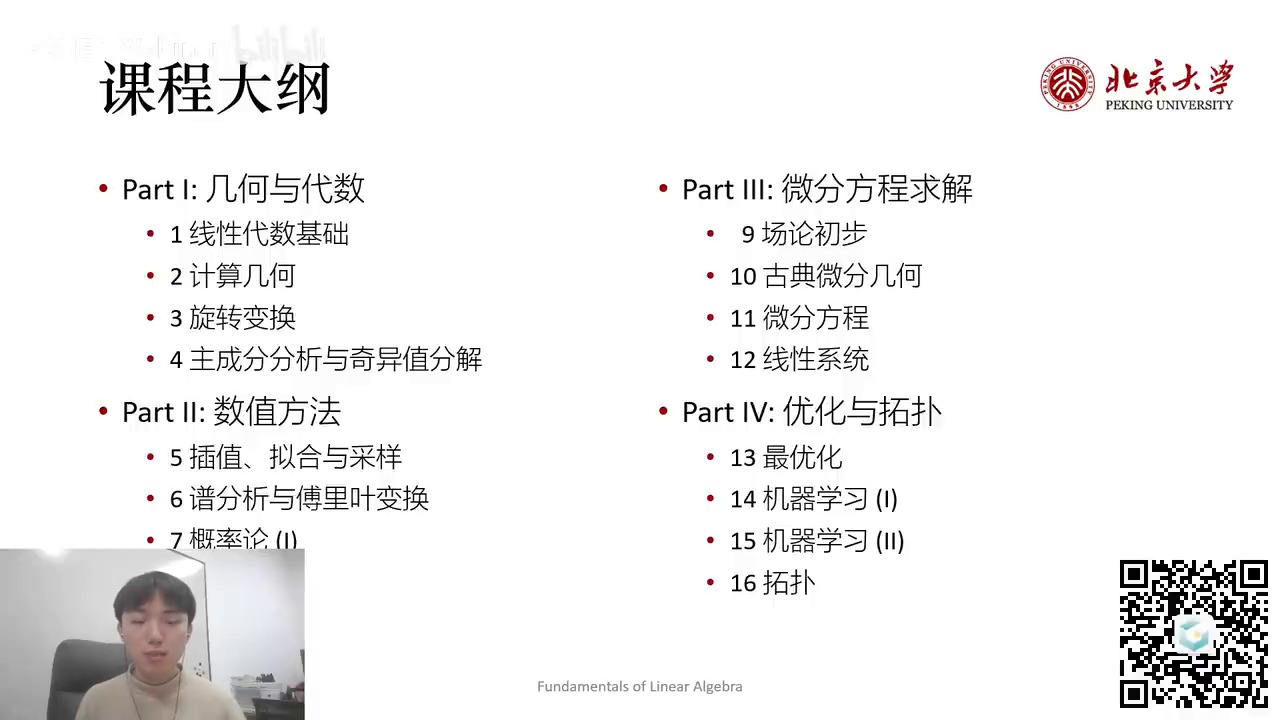
\includegraphics[width=0.92\textwidth]{figures/fig_01_syllabus.jpg}
\caption{课程大纲：几何与代数、数值方法、微分方程求解、优化与拓扑四个部分，共十六讲\vtag}
\end{figure}
\srcnote{00:14:30--00:14:45}
\end{minipage}


\subsection{世界模拟器：图形学的目标}

陈宝权老师开场抛出一个判断：计算机图形学的目标，是对现实世界做完全真实、逼真的仿真。近来大家讨论 Sora 是否构建了“世界模拟器”，所谓世界模拟器，就是对世界的运行能做高度精确的模拟：生成的场景物理真实，物体运动符合物理规律，人的动作符合人的行为，不会出现“穿帮”。图形学做到最好的状态，也正是在模拟世界；区别在于图形学的模拟有大量显式参数，而不像 Sora 那样输入一段文本即可。

\subsection{智能从哪里来：感知—认知—决策—行动的循环}

为了说明世界模拟器为何与人工智能密切相关，陈老师从“人的智能怎么来”说起。人类在成长中不断经历感知、认知、决策、行动，再回到感知，循环往复地积累经验。他用一个小朋友学倒水的视频说明：一开始倒得太快，水洒了；改成慢慢倒，水又顺着杯壁流出来；反复尝试后，终于学会“不快不慢”。在这个过程里，孩子并不知道术语，但他实际在学习容器的形状、水下落的物理规律，以及控制手部姿态的方法。

\noindent\begin{minipage}{\textwidth}
\begin{figure}[H]
\centering
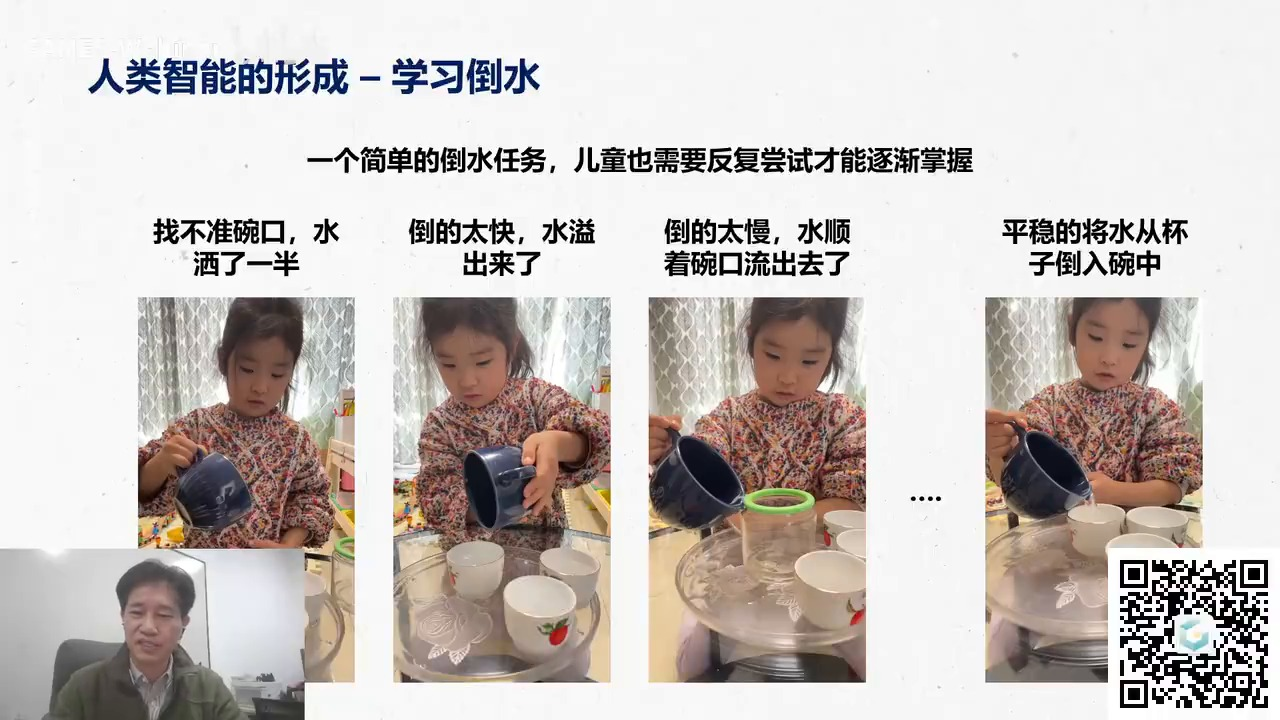
\includegraphics[width=0.92\textwidth]{figures/fig_02_child_pouring.jpg}
\caption{小朋友学倒水：太快会洒、太慢会顺杯壁流出，反复尝试后掌握恰当的速度\vtag}
\end{figure}
\srcnote{00:18:15--00:18:30}
\end{minipage}



\noindent\begin{minipage}{\textwidth}
\begin{figure}[H]
\centering
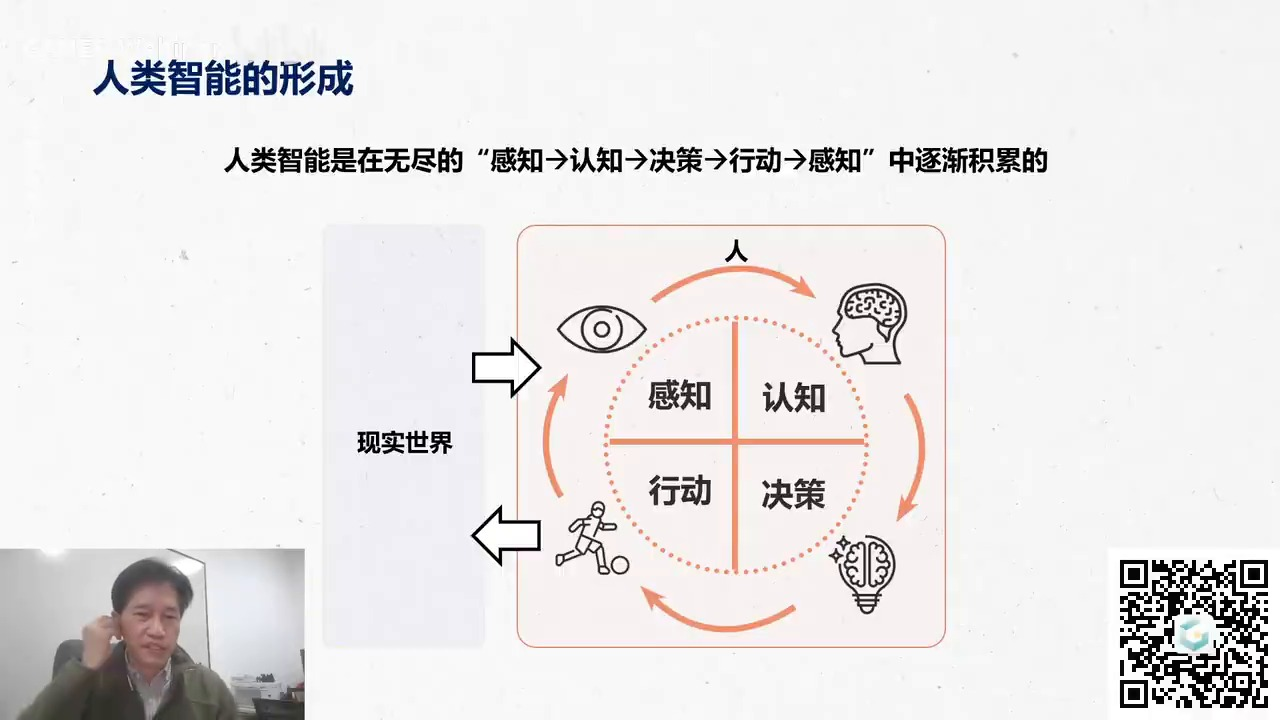
\includegraphics[width=0.92\textwidth]{figures/fig_03_perception_loop.jpg}
\caption{陈宝权老师用“感知—认知—决策—行动”的循环解释智能的来源\vtag}
\end{figure}
\srcnote{00:17:30--00:17:45}
\end{minipage}


如果让机器像人一样在现实世界里反复试错，效率很低：机器缺少人类与生俱来的生理基础，需要多得多的尝试，而且现实中的失败会造成真实的破坏。更好的办法是把现实世界变成数字世界，让智能体在数字世界里走同样的环路。数字世界可以“打碎了重来”，东西弄坏了也可以重置。构建这种与现实高度一致的数字世界的学科，就是计算机图形学。陈老师引用图灵奖得主 Ivan Sutherland 在 1965 年的设想：如果屏幕上展示的数字世界看起来是真的、交互起来是真的、听起来和摸起来也是真的，那么它就达到了图形学的最高境界。

\noindent\begin{minipage}{\textwidth}
\begin{figure}[H]
\centering
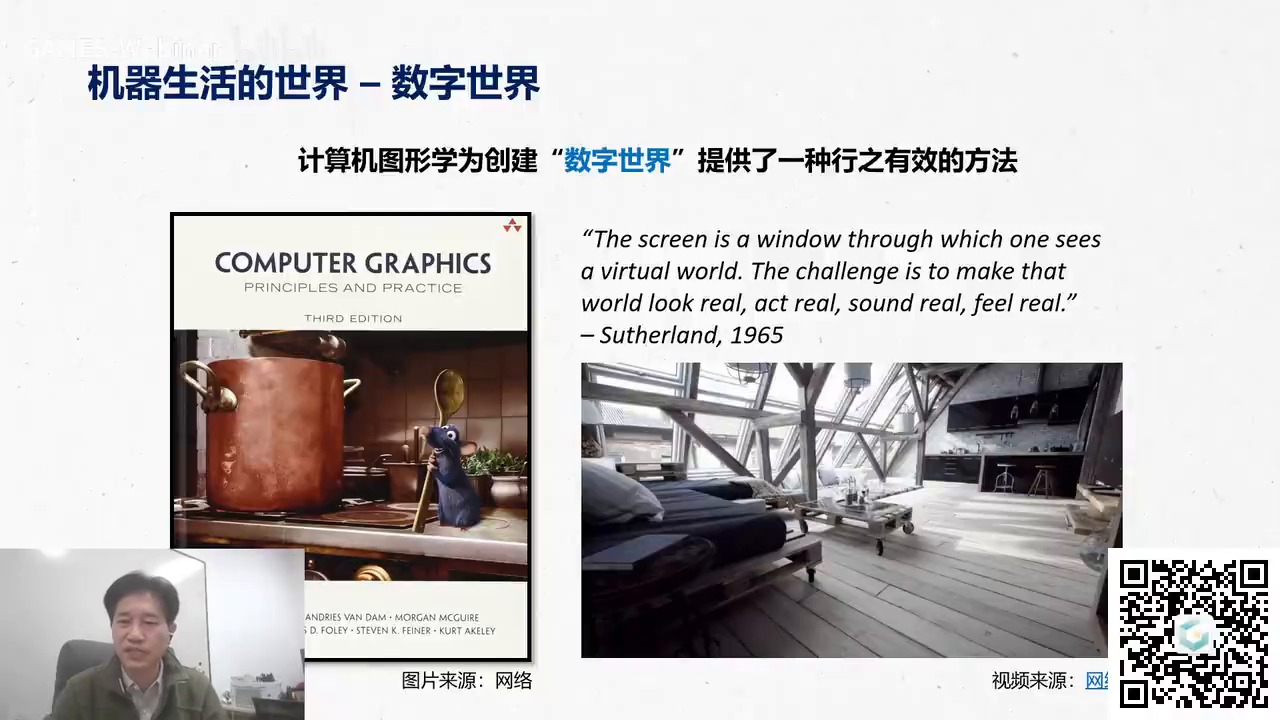
\includegraphics[width=0.92\textwidth]{figures/fig_04_sutherland_digital_world.jpg}
\caption{机器生活的世界是数字世界：Sutherland 在 1965 年设想的“终极显示”\vtag}
\end{figure}
\srcnote{00:22:15--00:22:30}
\end{minipage}



\begin{importantbox}{陈宝权老师的核心论点}
智能体在现实世界中学习既低效又昂贵；把现实世界数字化以后，智能体可以在数字世界中完成“感知—认知—决策—行动”的循环，并且可以无限次重来。图形学负责让这个数字世界在几何、物理与行为上都足够真实，因此它是训练智能体的基础设施。
\end{importantbox}

\subsection{构建数字世界需要哪些能力}

回到“让 AI 学倒水”的例子：首先要建立容器的几何形状；其次要有准确的流体动力学模拟，才能算出水怎样流下来；最后还需要可控的动作，模拟手抓杯子的过程。陈老师展示了他们实验室的若干工作：茶壶倒水、手部抓握动作的生成、在数字世界里叠一块布，以及煎鸡蛋、烘焙、切土豆等交互场景。他的推论是：如果交互模拟足够逼真，智能体与它交互时得到的反馈就与现实一致，它在数字世界里获得的经验也就能迁移到现实。



\noindent\begin{minipage}{\textwidth}
\begin{figure}[H]
\centering
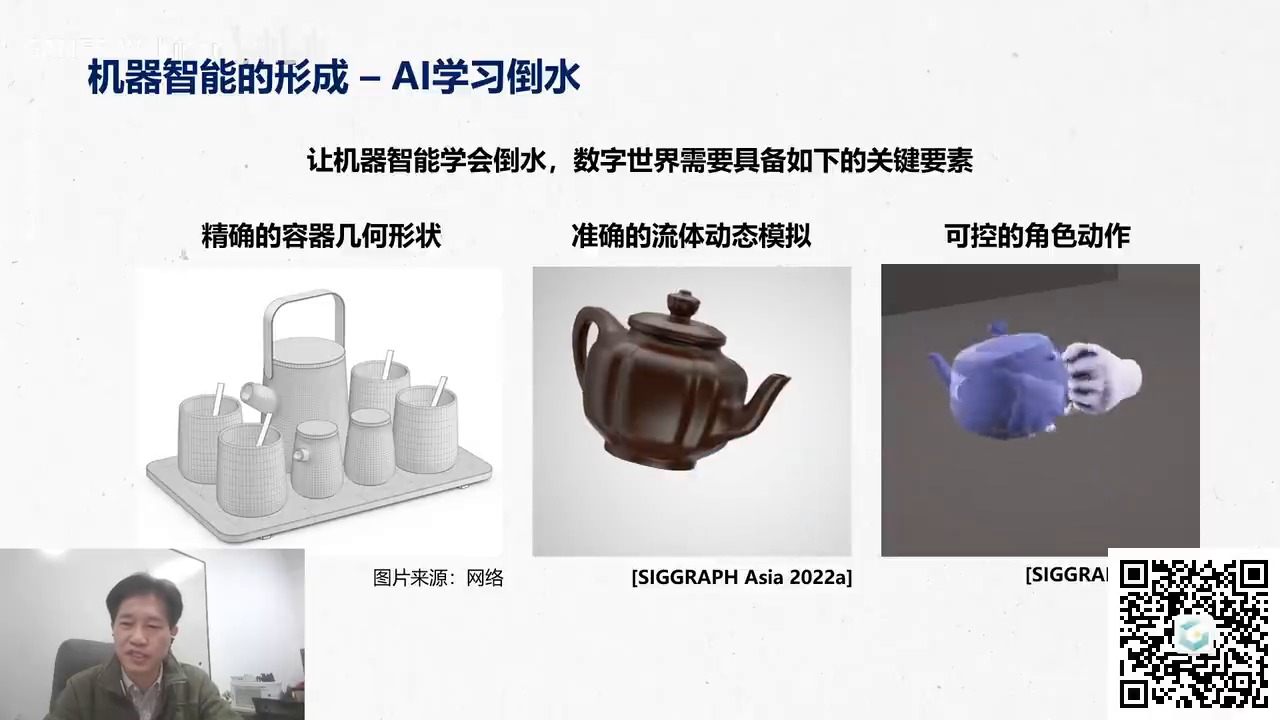
\includegraphics[width=0.92\textwidth]{figures/fig_05_digital_twin_tasks.jpg}
\caption{AI 学习倒水：数字世界需要提供精确的容器几何、流体动态与可控的手部动作\vtag}
\end{figure}
\srcnote{00:23:45--00:24:00}
\end{minipage}


\noindent\begin{minipage}{\textwidth}
\begin{figure}[H]
\centering
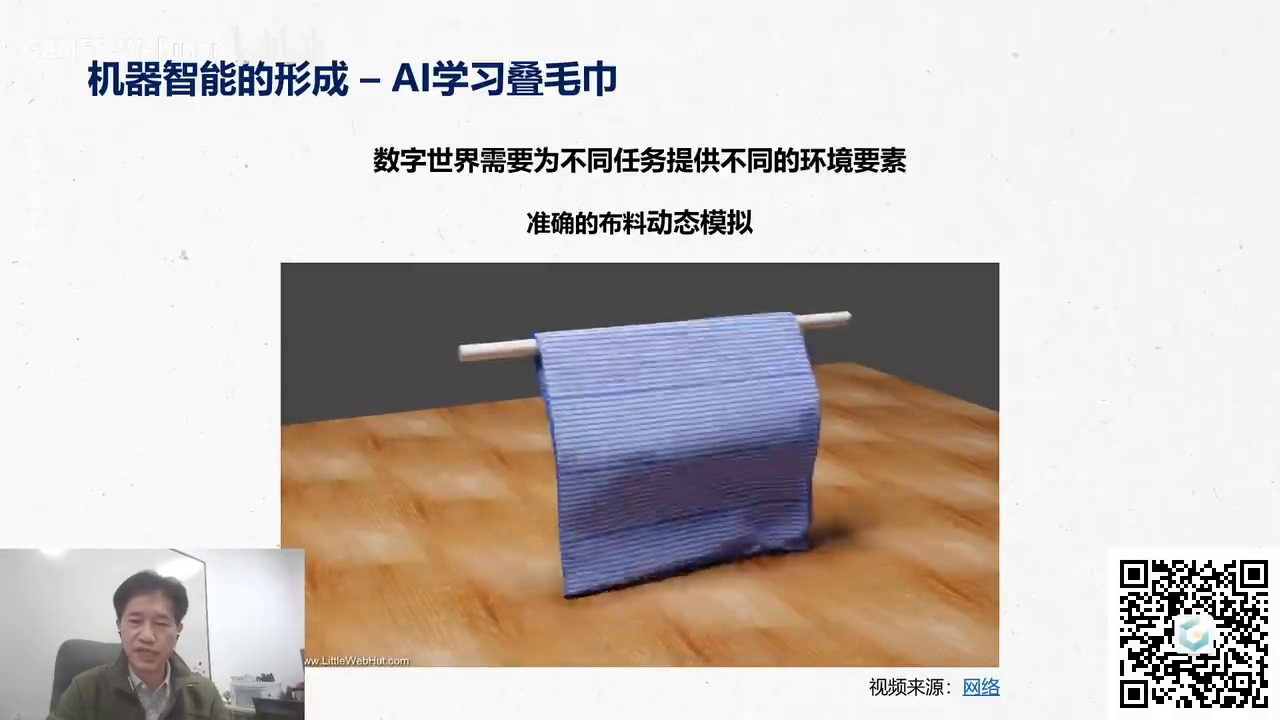
\includegraphics[width=0.92\textwidth]{figures/fig_06_cloth_folding.jpg}
\caption{AI 学习叠毛巾：数字世界需要为不同任务提供不同的环境要素\vtag}
\end{figure}
\srcnote{00:24:00--00:24:15}
\end{minipage}


\noindent\begin{minipage}{\textwidth}
\begin{figure}[H]
\centering
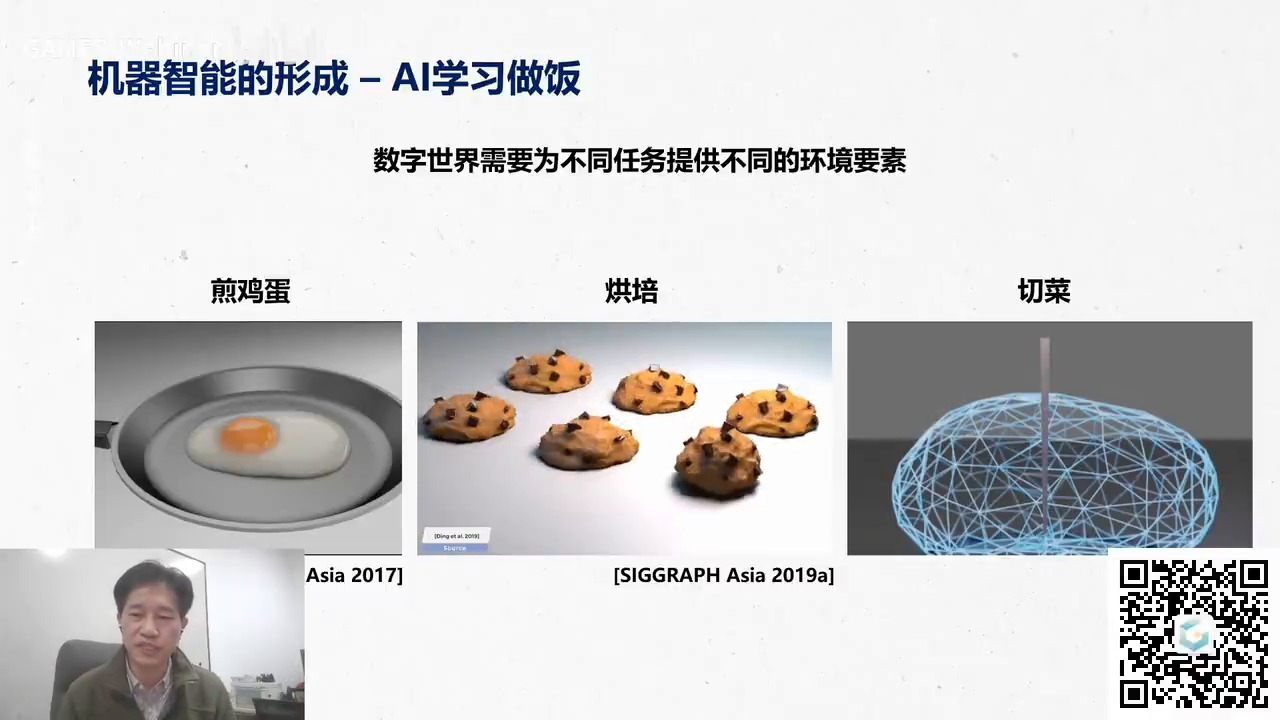
\includegraphics[width=0.92\textwidth]{figures/fig_07_cooking_tasks.jpg}
\caption{AI 学习做饭：煎鸡蛋、烘焙与切菜等任务分别需要不同的物理模拟\vtag}
\end{figure}
\srcnote{00:24:45--00:25:00}
\end{minipage}


\paragraph{几何的获取。}早期的三维形体主要靠交互式软件手工设计，效率不高，尤其难以得到现实世界中复杂的几何。另一条路线是直接把现实世界数字化：用传感设备测得三维点云，再用算法快速重建。陈老师介绍了他们早期的工作：地面上开着带传感器的车，或者让无人机在空中拍摄大量影像，重建出城市的三维模型；大约十年前，他们也用地面激光扫描直接获取点云。由此得到的建筑、树木等几何都来自精确测量，具备真实场景的复杂性。再往前一步，可以让机器人自己完成扫描：机器人一边观测、一边重建，还能根据“把场景完整重建”的目标判断哪里缺数据，再去补采；场景更大时，可以让多个机器人协同分工。陈老师还提到，央视《走进科学》曾有一期节目介绍过他们实验室的这项工作。陈老师强调，这些算法背后，正是本课程要讲的数学工具。

\noindent\begin{minipage}{\textwidth}
\begin{figure}[H]
\centering
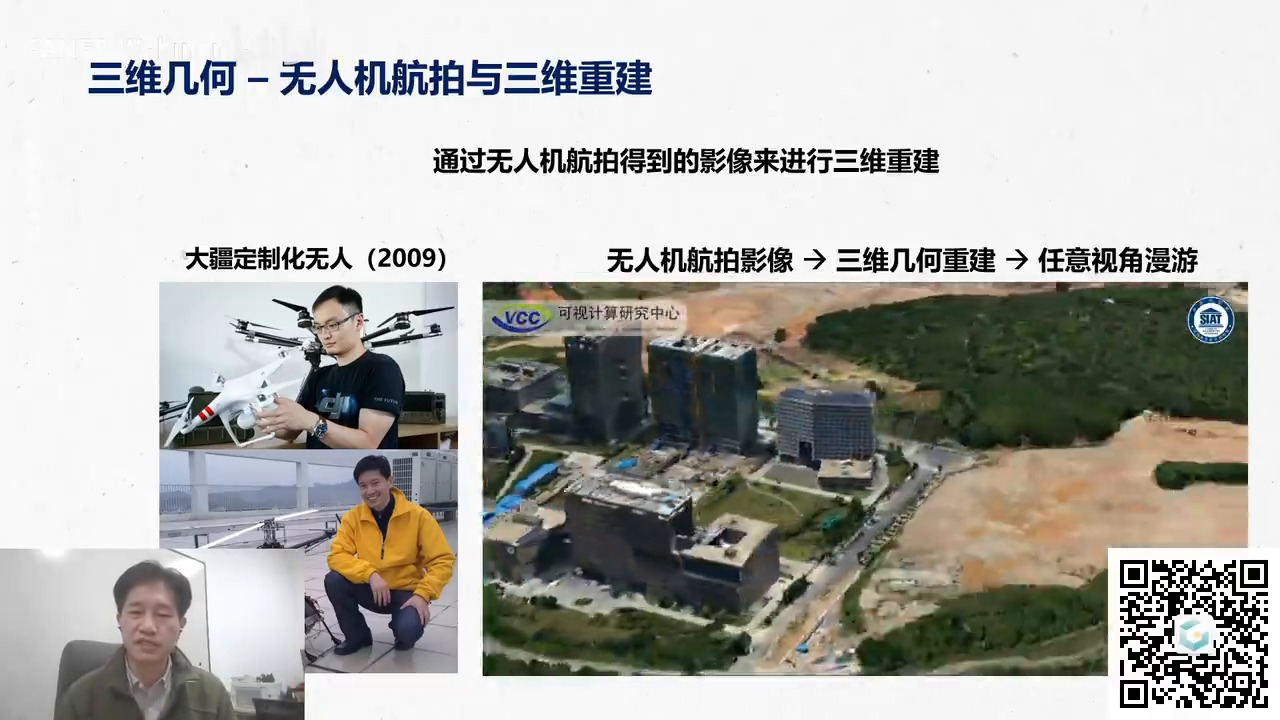
\includegraphics[width=0.92\textwidth]{figures/fig_08_scan_reconstruction.jpg}
\caption{无人机航拍与三维重建：通过大量影像恢复城市场景的三维几何\vtag}
\end{figure}
\srcnote{00:26:15--00:26:30}
\end{minipage}


\noindent\begin{minipage}{\textwidth}
\begin{figure}[H]
\centering
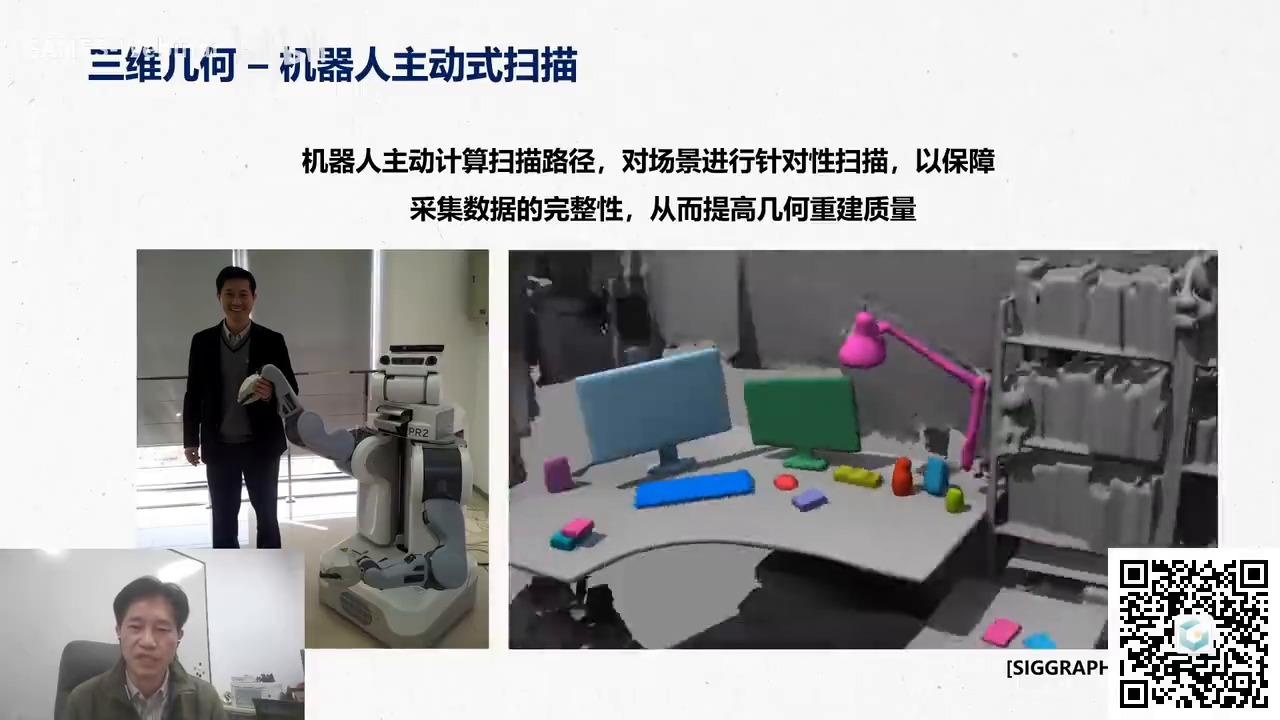
\includegraphics[width=0.92\textwidth]{figures/fig_09_robot_scanning.jpg}
\caption{机器人主动式扫描：机器人边观测、边重建，并主动去补采缺失的数据\vtag}
\end{figure}
\srcnote{00:28:00--00:28:15}
\end{minipage}


\noindent\begin{minipage}{\textwidth}
\begin{figure}[H]
\centering
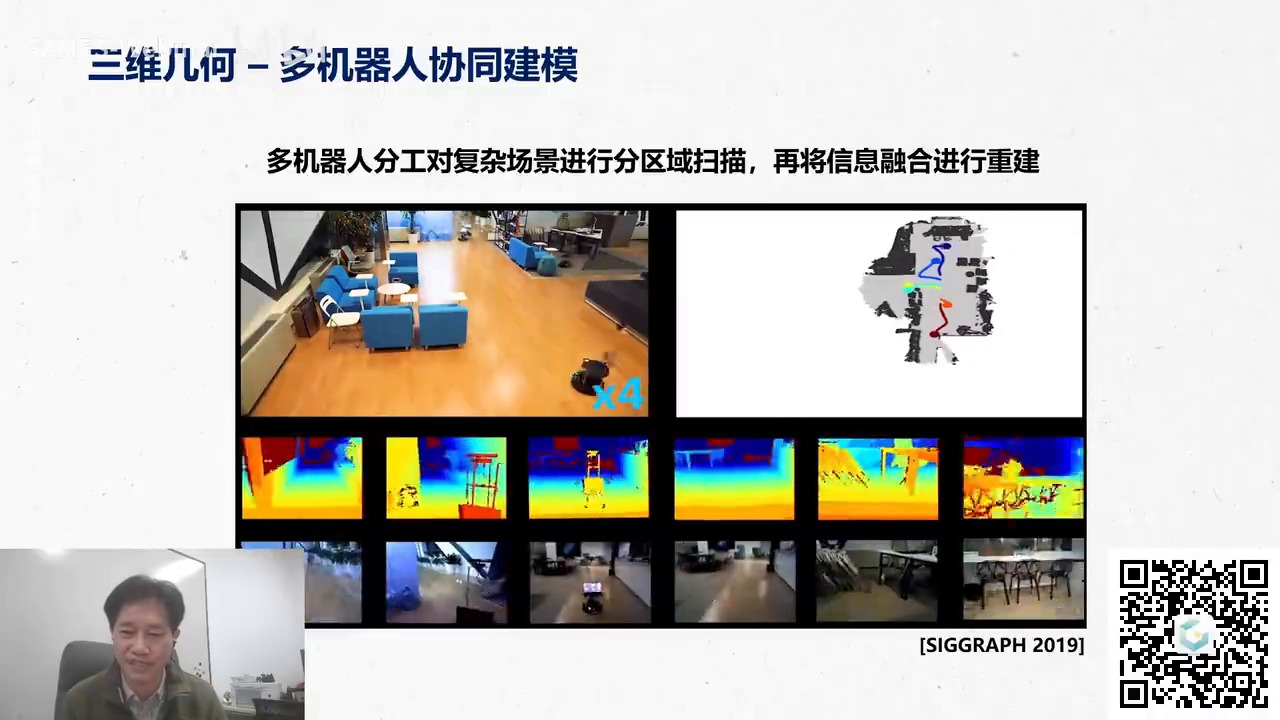
\includegraphics[width=0.92\textwidth]{figures/fig_10_multi_robot.jpg}
\caption{多机器人协同建模：多个机器人分工合作，重建更大、更复杂的场景\vtag}
\end{figure}
\srcnote{00:28:45--00:29:00}
\end{minipage}


\paragraph{物理仿真。}我们判断一个世界是否真实，很大程度上取决于其中的动态现象是否符合物理规律。陈老师列举了图形学算法能够模拟的现象：弹性与黏弹性体（如雪、奶油）、大尺度形变、数字人身上衣服的褶皱（薄壳类物体）、水、烟雾与液膜等流体。这些现象的模拟目标是“以假乱真”。他特别提到实验室几位同学的工作：固体落入液体这种多材质、多物态耦合的场景，倪星宇做的磁流体模拟，以及在外部磁场驱动下运动的薄壳软体机器人。后者没有电机，完全依靠磁场改变其形变，从而在液体里游动或在坡面上爬行；这类模拟对设计进入血管的微型医疗机器人很重要。

\noindent\begin{minipage}{\textwidth}
\begin{figure}[H]
\centering
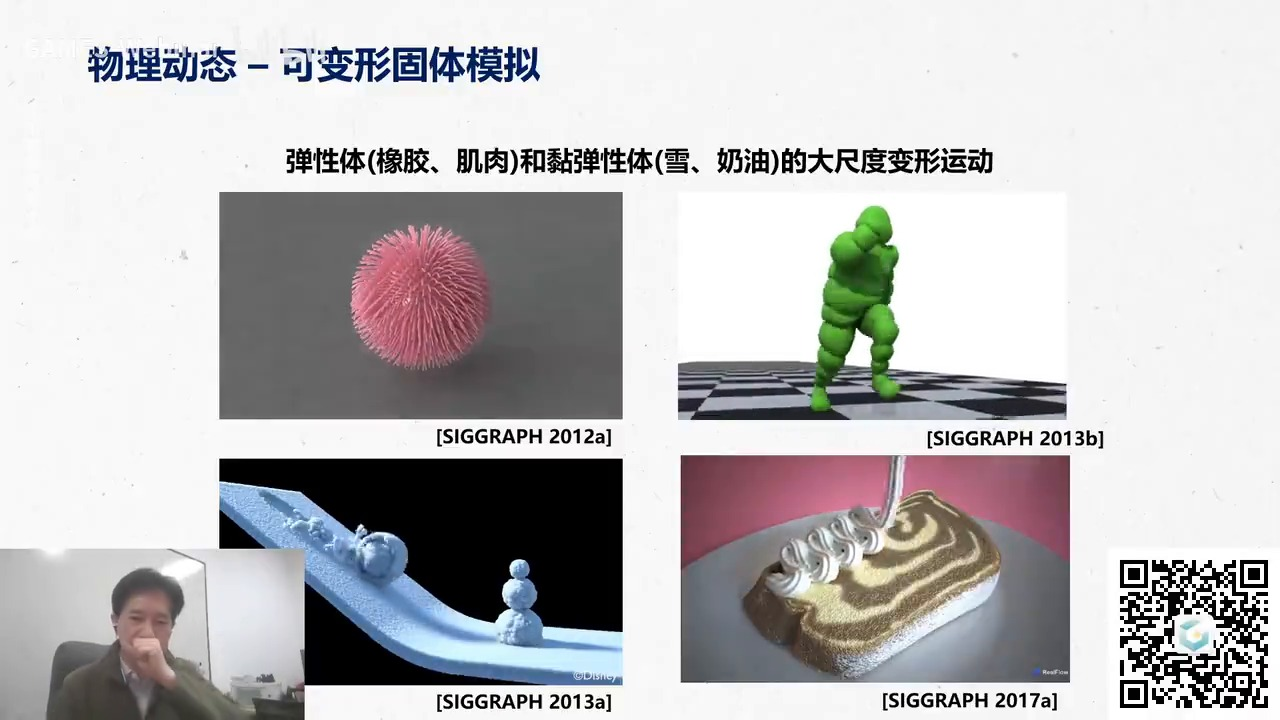
\includegraphics[width=0.92\textwidth]{figures/fig_11_physics_simulation.jpg}
\caption{可变形固体模拟：弹性体与黏弹性体（如雪、奶油）的大尺度形变\vtag}
\end{figure}
\srcnote{00:30:30--00:30:45}
\end{minipage}


\noindent\begin{minipage}{\textwidth}
\begin{figure}[H]
\centering
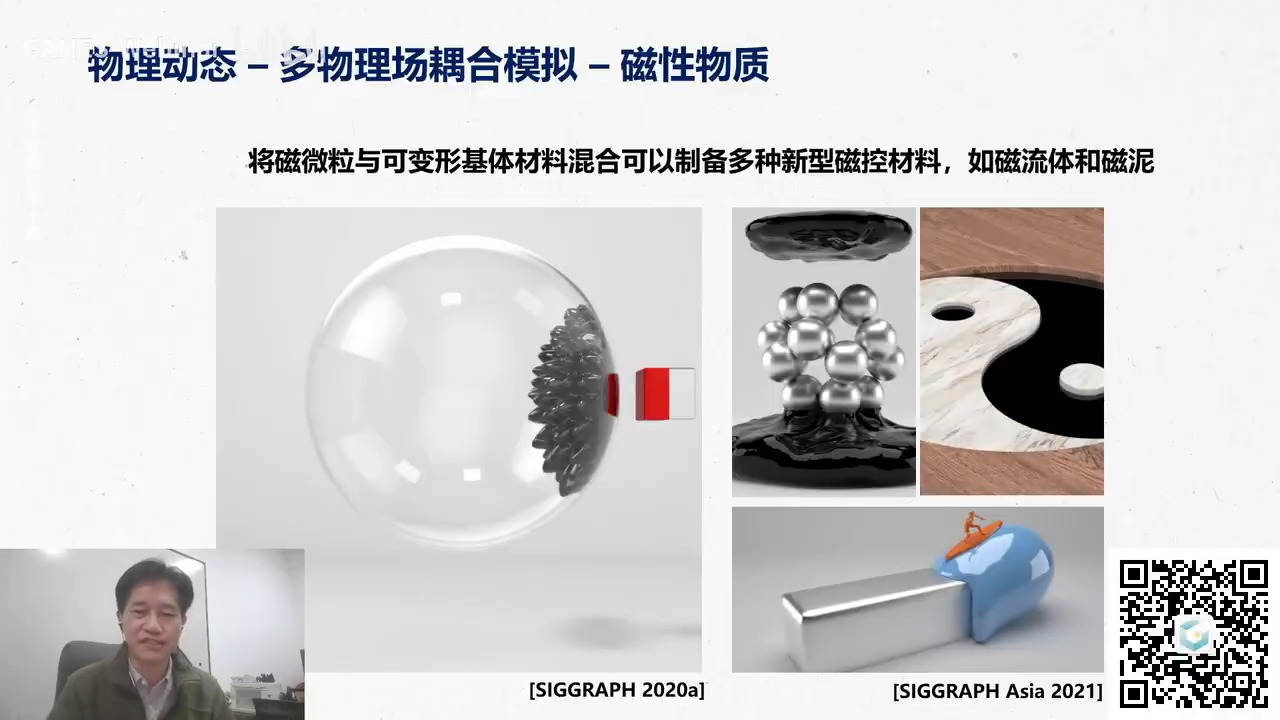
\includegraphics[width=0.92\textwidth]{figures/fig_12_ferrofluid.jpg}
\caption{多物理场耦合模拟：磁流体在外加磁场下形成的形态\vtag}
\end{figure}
\srcnote{00:32:30--00:32:45}
\end{minipage}


\noindent\begin{minipage}{\textwidth}
\begin{figure}[H]
\centering
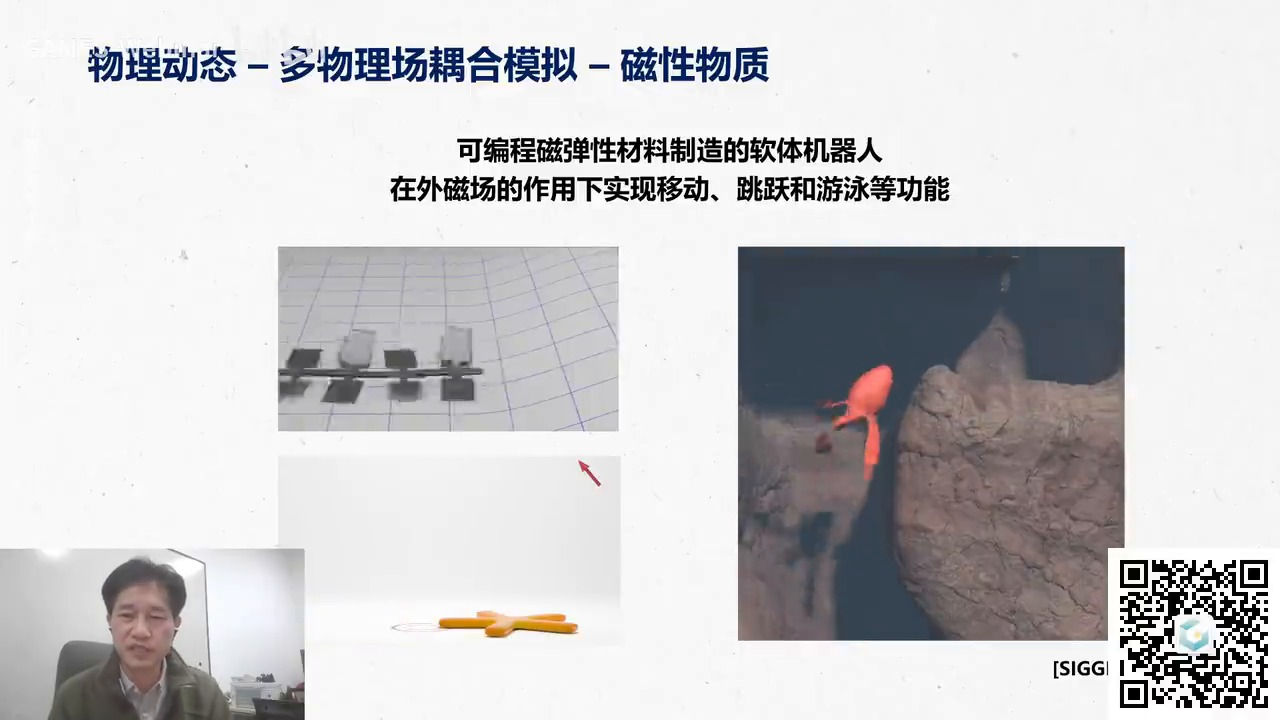
\includegraphics[width=0.92\textwidth]{figures/fig_13_soft_robot.jpg}
\caption{磁驱动的薄壳软体机器人：通过改变外部磁场，使其在液体中游动或在坡面上爬行\vtag}
\end{figure}
\srcnote{00:33:45--00:34:00}
\end{minipage}


\paragraph{从现实中“反求”物理。}正如几何可以从现实中扫描获得，物理现象也可以从现实中捕获。陈老师举了荷叶的例子：风吹动荷叶时把它的形变拍下来，再做物理过程的“反演”，恢复它的几何、材质与物理参数；得到这些描述以后，就能前向模拟它在新的外力（洒下的水珠、另一阵风）作用下的反应。烟雾也一样：用多个视角的视频捕获上升的烟，反演出密度场与速度场，烟就被“数字化”了，可以继续前向模拟。这里的数字化不只是形状，而是物体材质与物理属性的整体数字化。

\noindent\begin{minipage}{\textwidth}
\begin{figure}[H]
\centering
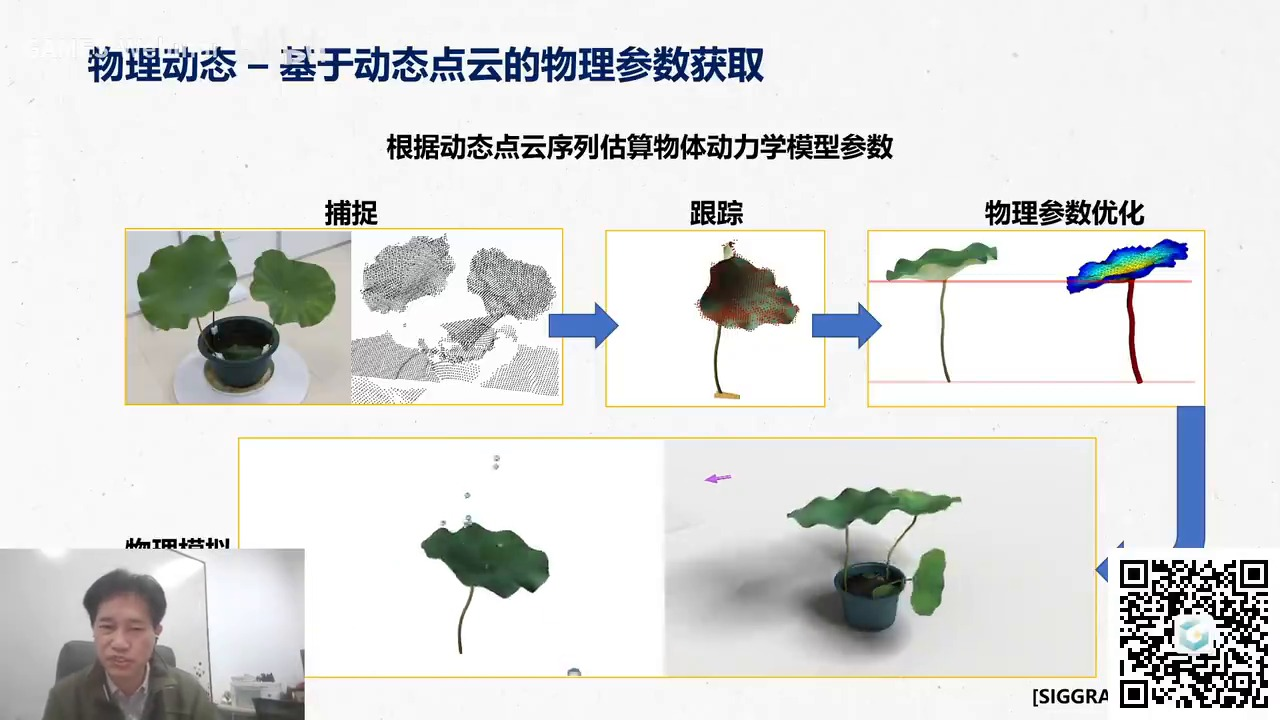
\includegraphics[width=0.92\textwidth]{figures/fig_14_inverse_physics.jpg}
\caption{基于点云的物理参数获取：捕获荷叶形变，反演其物理参数，再在新的外力下前向模拟\vtag}
\end{figure}
\srcnote{00:35:30--00:35:45}
\end{minipage}


\noindent\begin{minipage}{\textwidth}
\begin{figure}[H]
\centering
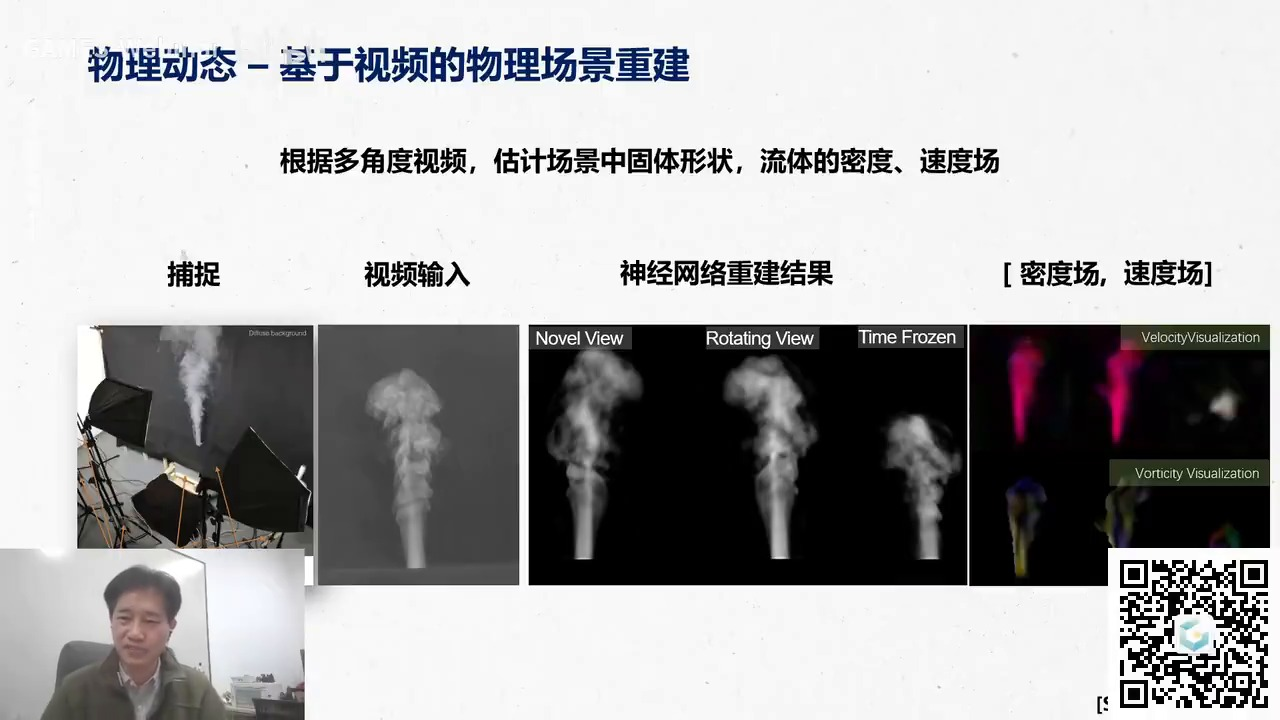
\includegraphics[width=0.92\textwidth]{figures/fig_15_smoke_capture.jpg}
\caption{基于视频的物理场景重建：从多视角视频反演烟雾的密度场与速度场\vtag}
\end{figure}
\srcnote{00:36:15--00:36:30}
\end{minipage}


\paragraph{人体运动与可学习的角色。}自然界中另一类重要的动态对象是人体。要让虚拟角色的动作看起来真实，需要先从视频中重建三维骨架运动。输入只是二维视频，重建出的三维运动却必须物理正确，否则学到的动作也是错的；因此重建过程反过来利用了图形学对骨架运动的物理约束。学到大量动作以后，可以驱动高矮胖瘦不同的新形体，还要保留个人风格这样的微妙差异。更进一步，角色具有自我学习能力：在数字环境中通过不断尝试（有同学在弹幕中指出这就是强化学习），从不会做动作到逐渐学会。陈老师承认这些工作越来越与人工智能交叉，两者相互促进。

\noindent\begin{minipage}{\textwidth}
\begin{figure}[H]
\centering
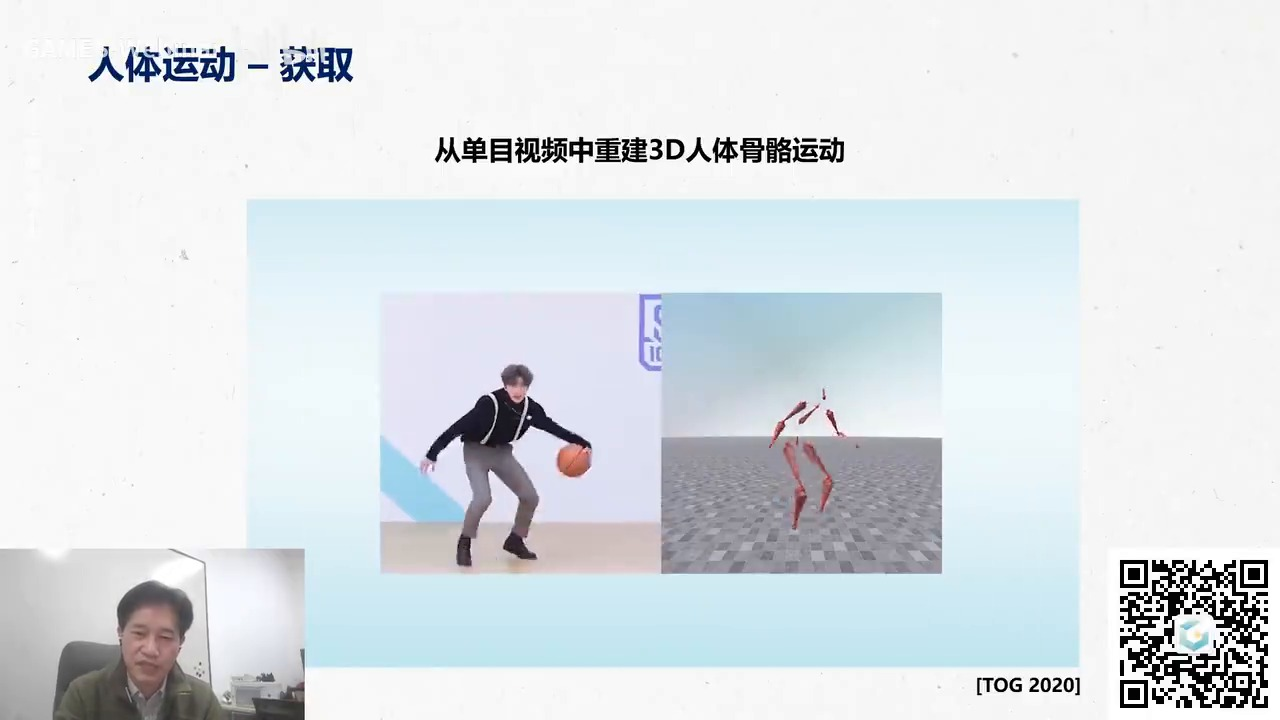
\includegraphics[width=0.92\textwidth]{figures/fig_16_motion_reconstruction.jpg}
\caption{人体运动获取：从单目视频中重建三维人体骨架运动\vtag}
\end{figure}
\srcnote{00:37:45--00:38:00}
\end{minipage}


\paragraph{虚实融合。}陈老师接着介绍了把人与虚拟世界连接起来的工作：借助各种虚拟现实/增强现实（VR/AR）设备，把真人的动作引入数字世界，使真实世界与数字世界之间形成一致的环路；真人表演与数字合成结合，数字世界与真人之间不断交互，生成越来越丰富的内容。

\noindent\begin{minipage}{\textwidth}
\begin{figure}[H]
\centering
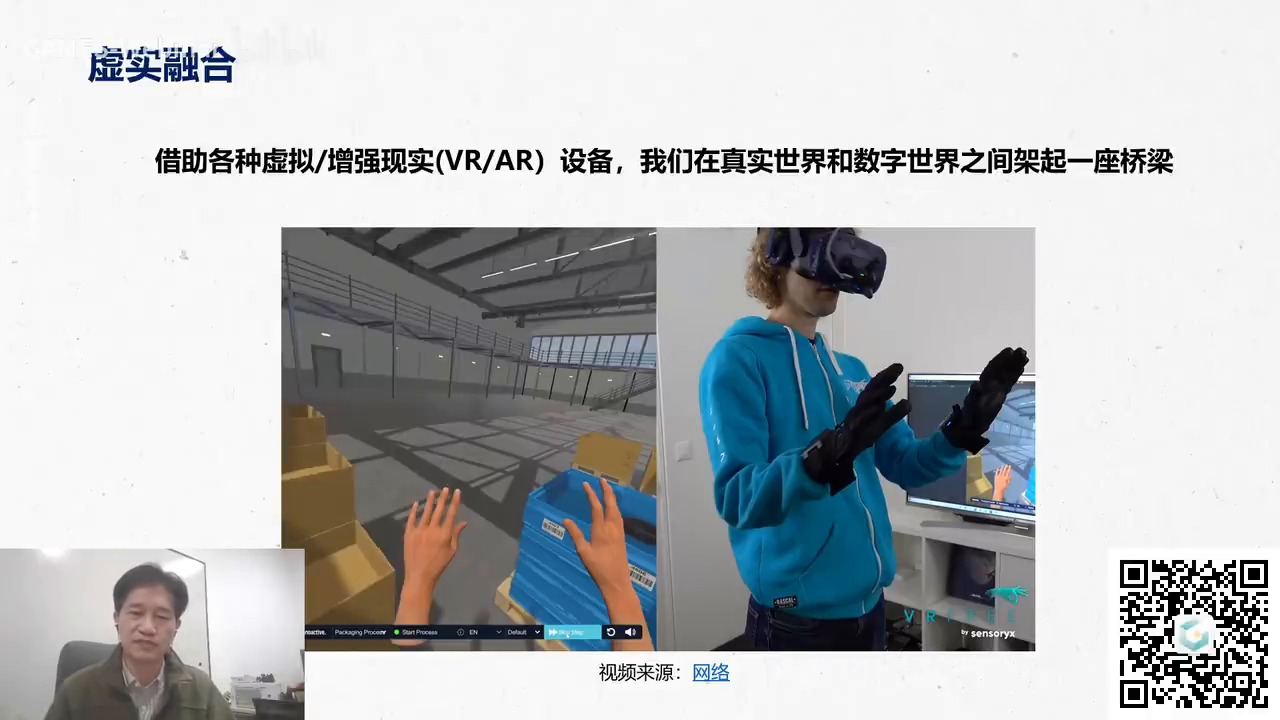
\includegraphics[width=0.92\textwidth]{figures/fig_17_vr_fusion.jpg}
\caption{虚实融合：借助 VR/AR 设备，让真实世界与数字世界之间形成一致的交互环路\vtag}
\end{figure}
\srcnote{00:43:15--00:43:30}
\end{minipage}


\subsection{具身智能与自动驾驶：在数字世界里训练}

陈老师最后回到应用。以自动驾驶为例：一个能力不足的智能驾驶系统不能直接上街，这是第一；第二，现实中能跑的场景是有限的。数字世界则不同，路面、天气、交通状况都可以随意改变，系统在数字世界里学好本事，再部署到物理的车上。机器人也一样，从设计外形开始就要模拟它的行走能力。他还提到正在开发的“大任务平台”：在一个有许多行人的街道与社会系统中训练智能体，不断扩充其能力。

\noindent\begin{minipage}{\textwidth}
\begin{figure}[H]
\centering
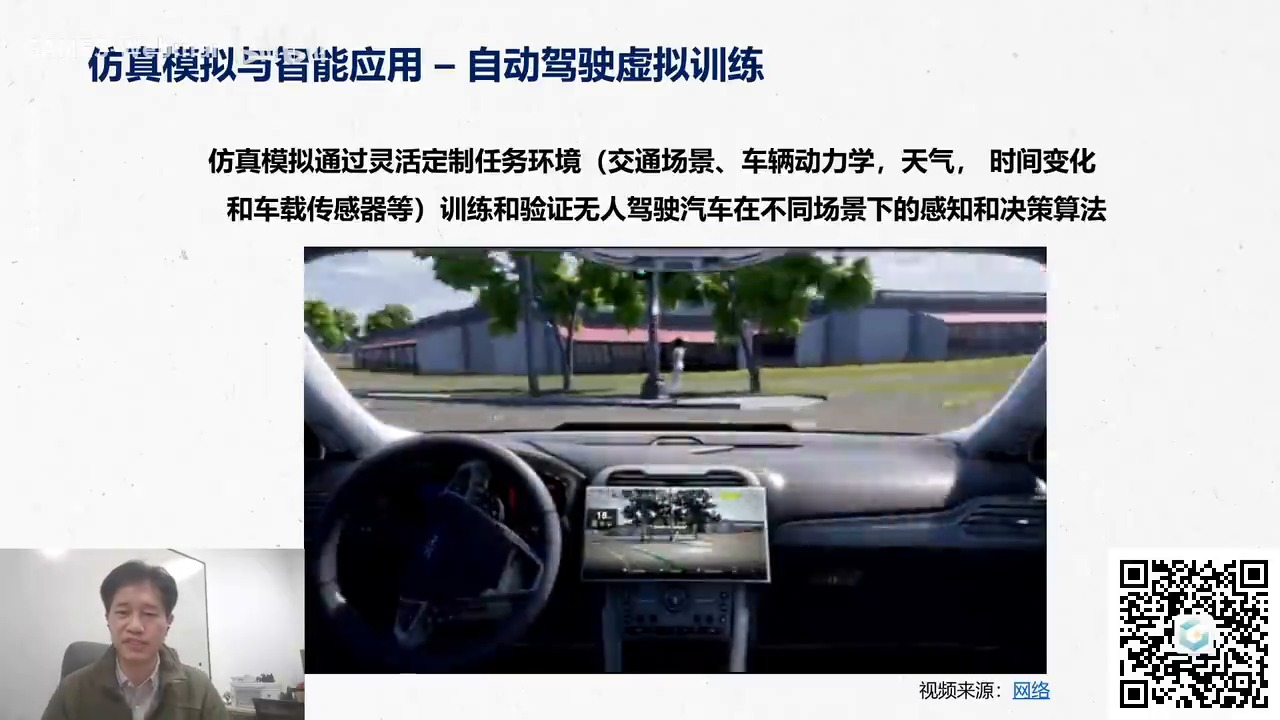
\includegraphics[width=0.92\textwidth]{figures/fig_18_embodied_training.jpg}
\caption{仿真模拟与智能应用：在数字世界中训练自动驾驶的感知与决策，场景、天气与交通可以任意改变\vtag}
\end{figure}
\srcnote{00:45:30--00:45:45}
\end{minipage}


\noindent\begin{minipage}{\textwidth}
\begin{figure}[H]
\centering
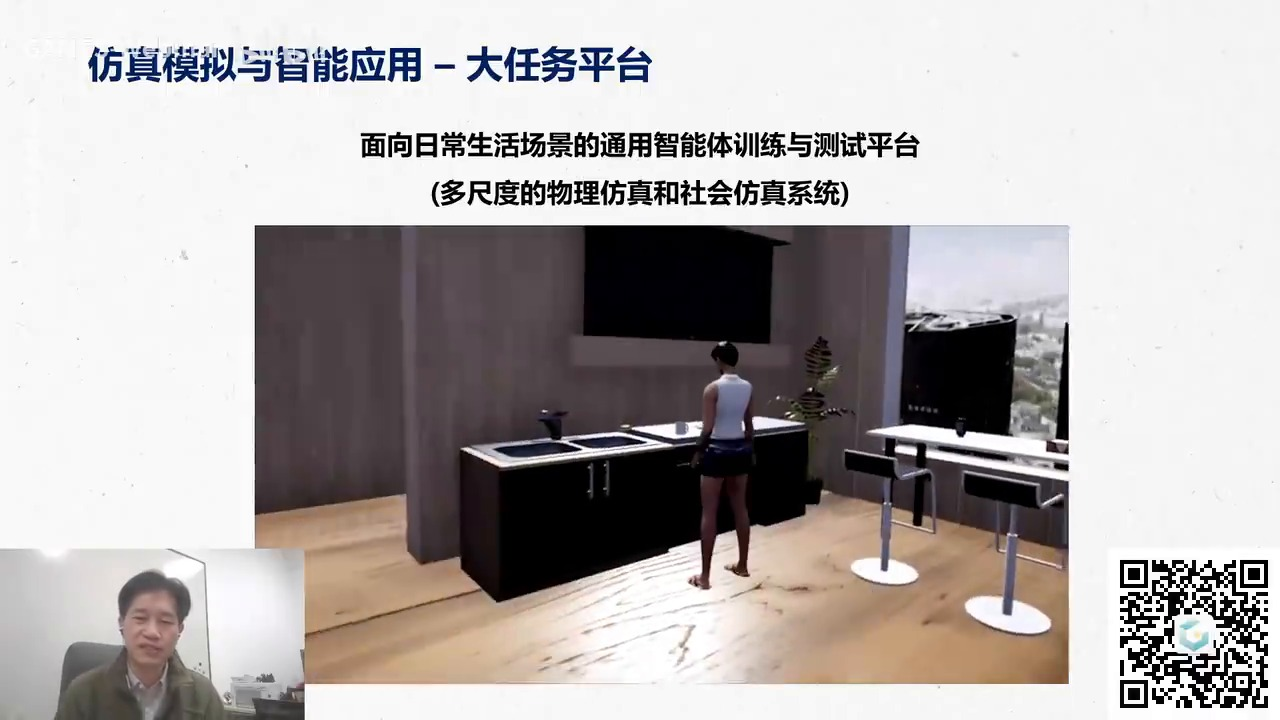
\includegraphics[width=0.92\textwidth]{figures/fig_19_task_platform.jpg}
\caption{面向日常生活场景的通用智能体训练与测试平台（大任务平台）\vtag}
\end{figure}
\srcnote{00:48:30--00:48:45}
\end{minipage}


课件在这里引用了费曼的名言“What I cannot create, I do not understand”。陈老师的结语是：我们之所以能够生成世界，是因为我们理解了世界；生成世界又反过来帮助我们更好地理解世界，两者相互促进。而支撑这一切的，是一个好的数学工具箱，这也正是这门课要提供的东西。

\noindent\begin{minipage}{\textwidth}
\begin{figure}[H]
\centering
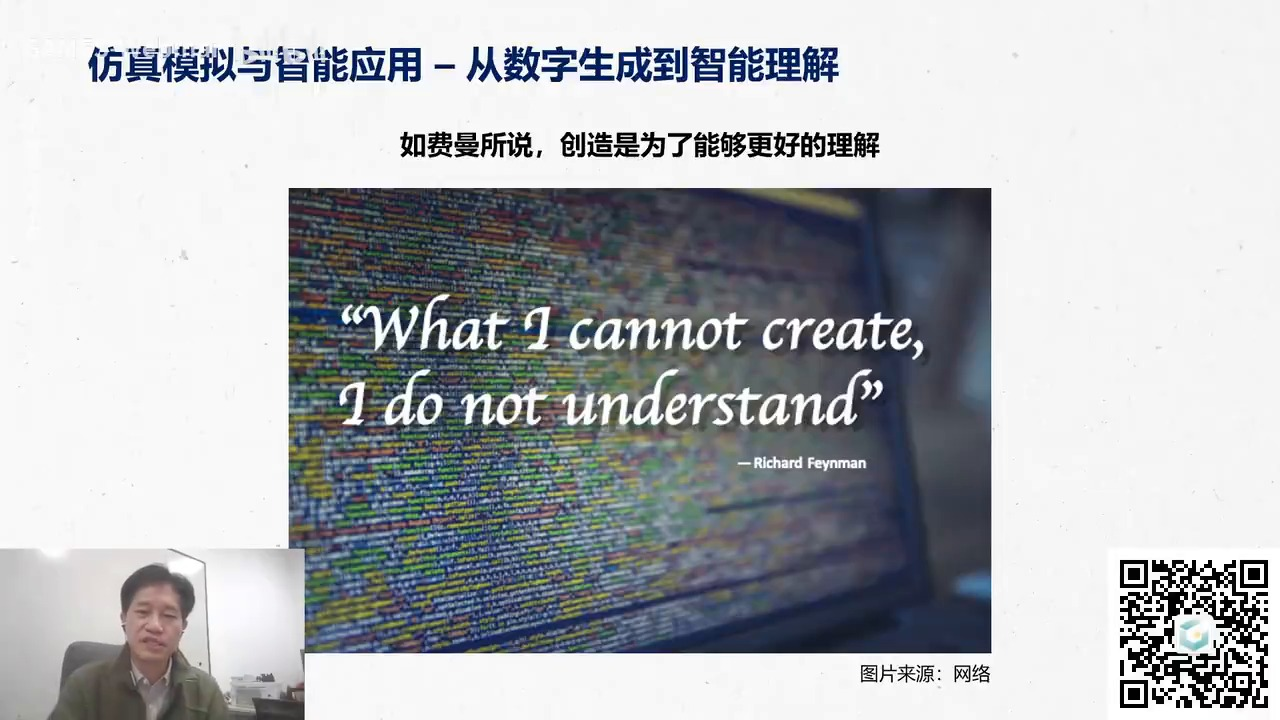
\includegraphics[width=0.92\textwidth]{figures/fig_20_create_understand.jpg}
\caption{从数字生成到智能理解：课件引用费曼的名言“What I cannot create, I do not understand”\vtag}
\end{figure}
\srcnote{00:50:15--00:50:30}
\end{minipage}


\subsection{本章小结}

第一章回答了“为什么要学图形学中的数学”：图形学的目标是逼真地模拟世界，几何获取、物理仿真、物理反演、运动重建以及智能体训练，都建立在数学工具之上。接下来的线性代数部分是这个工具箱的第一层，因为图形学处理的基本对象（位置、法向、颜色乃至整个模型的状态）本质上都是向量。

\section{向量与向量空间：图形学处理的基本对象}

倪星宇首先说明了讲法上的选择。大学线性代数通常用一整个学期讲完，许多教材从行列式切入；这门课只有一两讲的时间，所以选择和国外教材一样从向量讲起，让读者最快地明白线性代数研究什么问题、想达到什么目的。对图形学来说，这种讲法更加贴切：无论是点的位置还是法向，它们本质上都是向量。

\subsection{两种“向量”}

读者脑中大概有两种向量。第一种来自中学数学与物理：既有大小又有方向的量（物理上称矢量），运算满足平行四边形法则，即两个向量 $\boldsymbol v$ 与 $\boldsymbol w$ 相加，结果是以它们为邻边的平行四边形的对角线。第二种来自线性代数：向量是向量空间（线性空间）中的元素，它们之间的运算满足一组公理化定义。

\noindent\begin{minipage}{\textwidth}
\begin{figure}[H]
\centering
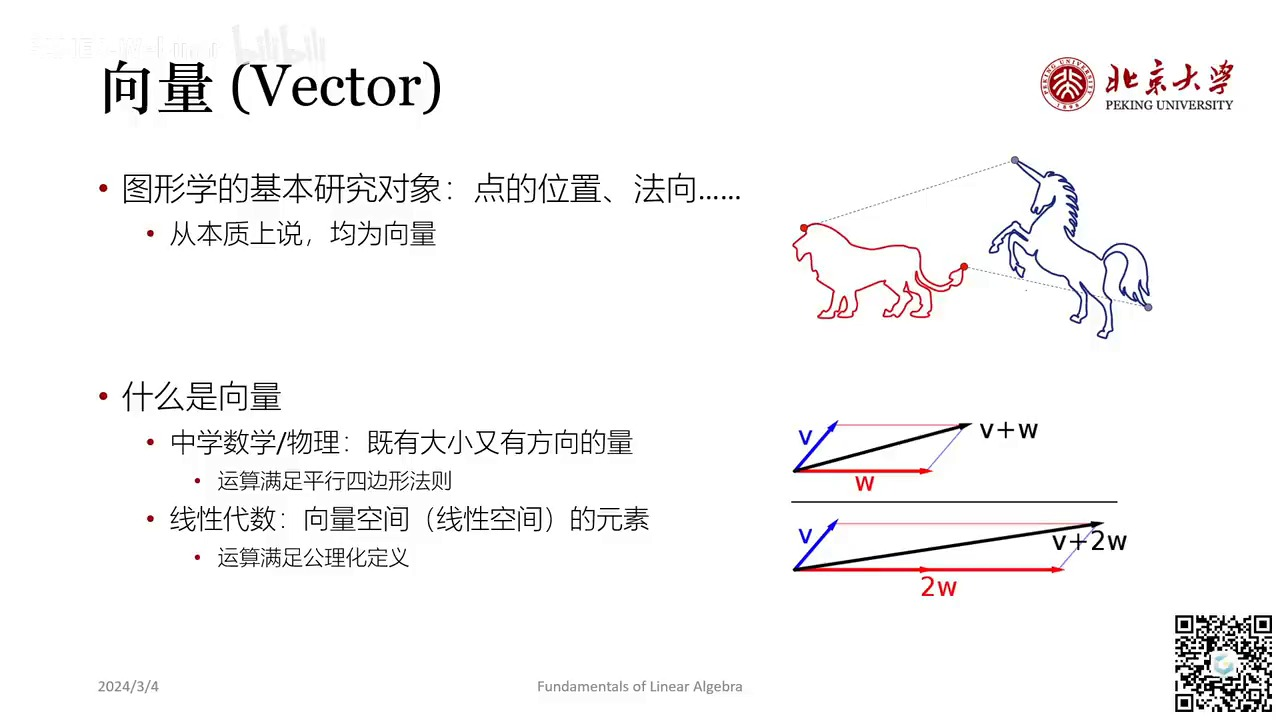
\includegraphics[width=0.92\textwidth]{figures/fig_21_vector_intro.jpg}
\caption{向量的两种理解：中学的“有大小有方向的量”与线性代数中向量空间的元素\vtag}
\end{figure}
\srcnote{00:56:45--00:57:00}
\end{minipage}


\subsection{向量空间的公理}

公理化定义是这样的：给定数域 $F$，$F$ 上的向量空间是一个带有向量加法与标量乘法的非空集合 $V$，对任意 $\boldsymbol u,\boldsymbol v,\boldsymbol w\in V$ 与 $a,b\in F$，满足以下八条：
\[
\begin{aligned}
&\boldsymbol u+(\boldsymbol v+\boldsymbol w)=(\boldsymbol u+\boldsymbol v)+\boldsymbol w, &\quad& \boldsymbol u+\boldsymbol v=\boldsymbol v+\boldsymbol u,\\
&\boldsymbol v+\boldsymbol 0=\boldsymbol v, && \boldsymbol v+(-\boldsymbol v)=\boldsymbol 0,\\
&a(b\boldsymbol v)=(ab)\boldsymbol v, && 1\boldsymbol v=\boldsymbol v,\\
&a(\boldsymbol u+\boldsymbol v)=a\boldsymbol u+a\boldsymbol v, && (a+b)\boldsymbol v=a\boldsymbol v+b\boldsymbol v .
\end{aligned}
\]
\begin{itemize}
\item $\boldsymbol u,\boldsymbol v,\boldsymbol w$：$V$ 中的向量；$\boldsymbol 0$：加法单位元（零向量）；$-\boldsymbol v$：$\boldsymbol v$ 的加法逆元；
\item $a,b$：数域 $F$ 中的标量；$1$：$F$ 的乘法单位元。
\end{itemize}
这八条依次是：加法结合律、加法交换律、加法单位元、加法逆元、标量乘法与数域乘法的结合律、标量乘法单位元、标量乘法对向量加法的分配律、标量乘法对数域加法的分配律。在图形学应用中，数域 $F$ 一般取实数域 $\mathbb R$，也可以选择复数域 $\mathbb C$ 等。

讲者强调，这种定义的最大好处在于：向量不一定要用坐标表达，它可以只是一个抽象概念。只要一个集合及其运算满足这八条，它就是向量空间，二维、三维的直观理解就可以平移到很高的维度上使用。

\begin{knowledgebox}{作业中的一个问题}
课件提出：颜色空间（RGB、CMYK）为什么也可以构成向量空间？要回答它，需要为颜色定义加法与标量乘法，并逐条检验上述八条公理。这道题留作课后作业。
\end{knowledgebox}

\subsection{本章小结}

向量空间是“满足八条公理的集合”，它不依赖坐标，也不限定维度。这一抽象让我们可以用同一套规则去处理位置、颜色、网格顶点乃至函数。下一步要回答：在这样的空间里，怎样用少数几个向量描述所有向量。

\section{线性组合、基与维度：图形学的问题有多大}

\subsection{线性相关与线性无关}

在向量集合 $\{\boldsymbol u_1,\boldsymbol u_2,\dots,\boldsymbol u_n\}$ 上，若数域 $F$ 中存在一组不全为 $0$ 的数 $a_1,\dots,a_n$ 使
\[
a_1\boldsymbol u_1+a_2\boldsymbol u_2+\cdots+a_n\boldsymbol u_n=\boldsymbol 0,
\]
\begin{itemize}
\item $\boldsymbol u_i$：集合中的第 $i$ 个向量；$a_i$：对应的组合系数；$\boldsymbol 0$：零向量，
\end{itemize}
就称这组向量线性相关；若不存在这样一组不全为零的数，则称线性无关。线性相关时，若 $a_1\neq 0$，可以把 $\boldsymbol u_1$ 解出来：
\[
\boldsymbol u_1=-\frac{a_2}{a_1}\boldsymbol u_2-\frac{a_3}{a_1}\boldsymbol u_3-\cdots-\frac{a_n}{a_1}\boldsymbol u_n ,
\]
\begin{itemize}
\item 右侧各项系数 $-a_i/a_1$ 都在数域 $F$ 中，因此 $\boldsymbol u_1$ 是 $\boldsymbol u_2,\dots,\boldsymbol u_n$ 的线性组合。
\end{itemize}
这说明“线性相关”的直观含义：其中某个向量可以由其余向量组合出来，是冗余的。

\subsection{维度、基与坐标}

在空间内能找出的线性无关向量个数的最大值，称为向量空间的维度，记作 $\dim V$（dim 是 dimension 的缩写）。$\dim V$ 个线性无关的向量构成空间的一组基（basis vectors），空间中任意向量都可以唯一地表示为这组基的线性组合，组合系数（coefficients）称为该向量在这组基下的坐标（coordinates）。唯一性可以用反证法得出：若某向量有两种不同的组合表示，两式相减，要么说明这组基线性相关，与假设矛盾，要么两种表示完全相同。

讲者指出，这样就避免了高中那种“先把向量定义为坐标组”的做法：坐标是在选定一组基之后才出现的，向量本身先于坐标存在。

\noindent\begin{minipage}{\textwidth}
\begin{figure}[H]
\centering
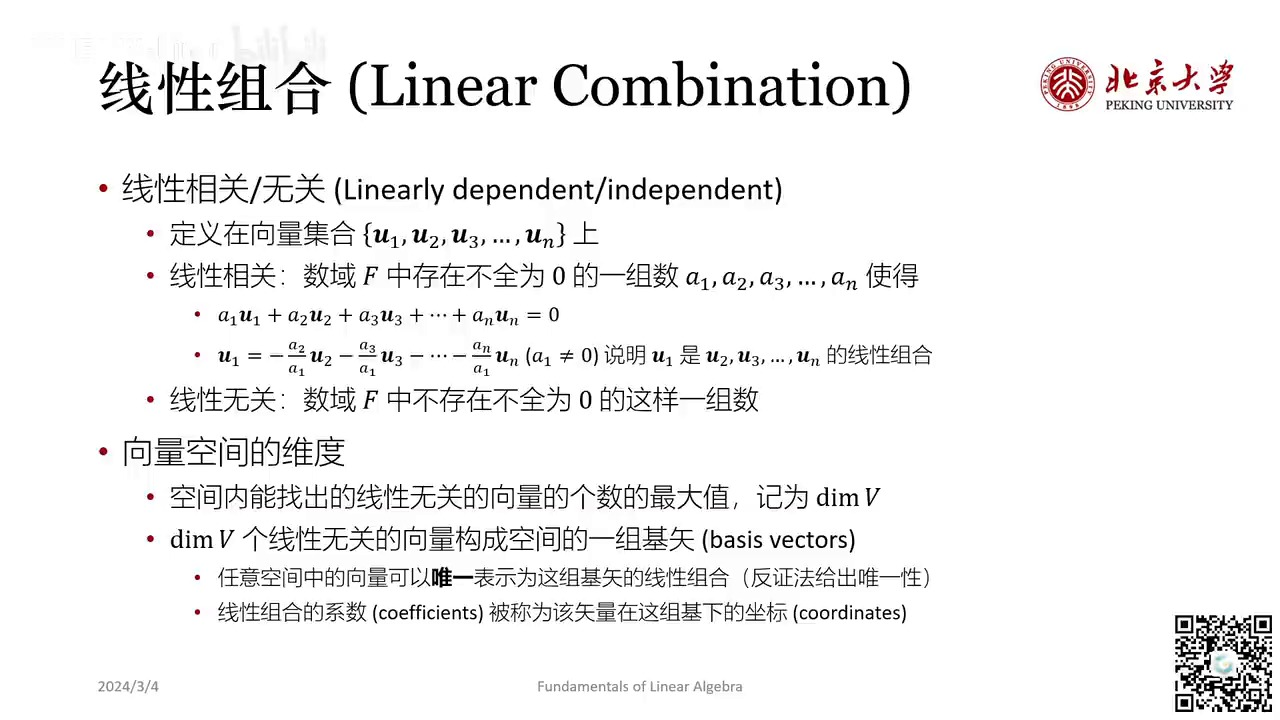
\includegraphics[width=0.92\textwidth]{figures/fig_22_linear_combination.jpg}
\caption{线性相关、线性无关、维度与基的定义\vtag}
\end{figure}
\srcnote{01:02:00--01:02:15}
\end{minipage}


\subsection{图形学研究的维度}

倪星宇把图形学研究的空间粗分为低维和高维两类。

\begin{itemize}
\item \textbf{低维（2D--4D）。}物理空间是图形学用得最多的空间：网格（mesh）、曲线、点云的坐标及其导数都在其中表达，例如欧几里得空间 $(x,y,z)$，以及相对论中的闵可夫斯基空间 $(x,y,z,ict)$。颜色空间（RGB、CMYK）也是重要的低维空间。
\item \textbf{高维。}一张 $1920\times1080$ 的灰度数字图像，把全部像素值排成一个向量，维度就达到约 200 万。二维或三维图形的全部自由度也可以组成一个向量：课件举了《原神》中纳西妲的模型，其运动顶点的自由度数为 45459。讲者解释，这是顶点数 15153 乘以 3 的结果。SIGGRAPH 上水体模拟求解的向量维度一般在 $10^6$ 到 $10^7$ 之间，讲者补充说，一些酷炫的效果需要一千万维的向量才能做到。
\end{itemize}

\noindent\begin{minipage}{\textwidth}
\begin{figure}[H]
\centering
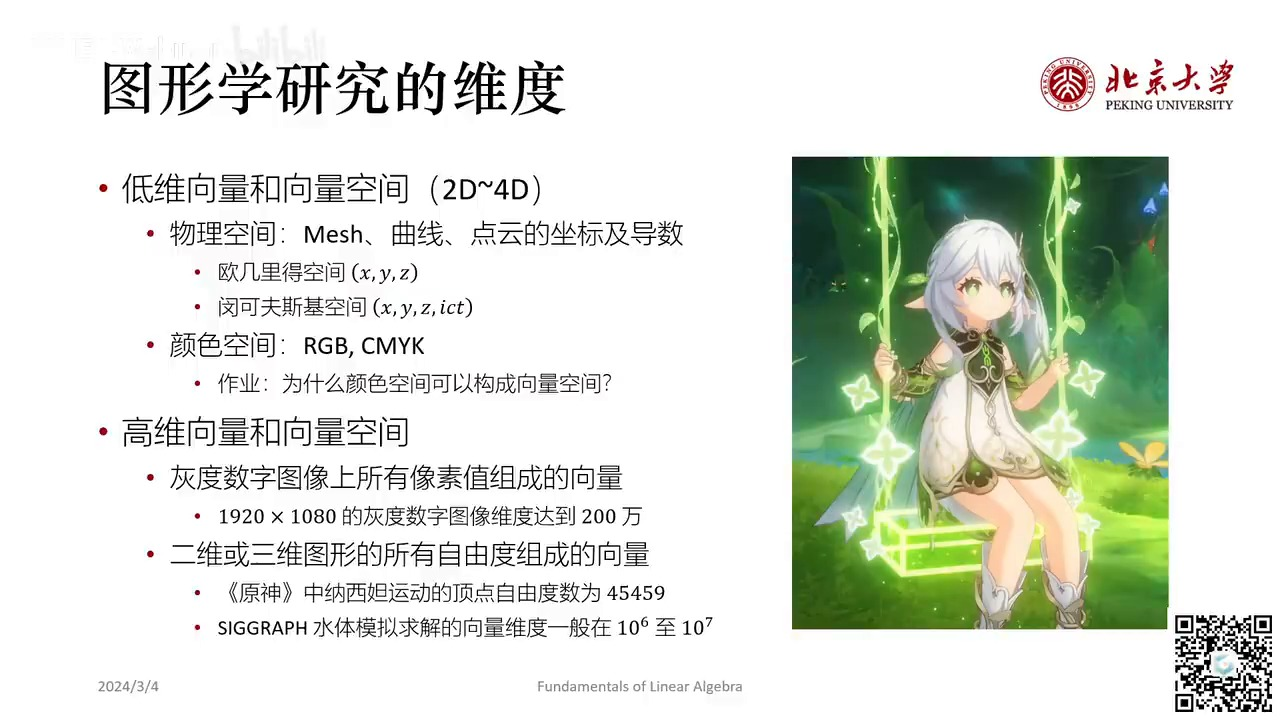
\includegraphics[width=0.92\textwidth]{figures/fig_23_graphics_dimensions.jpg}
\caption{图形学研究的维度：从 2D--4D 的物理与颜色空间，到百万维的图像与模拟状态\vtag}
\end{figure}
\srcnote{01:06:00--01:06:15}
\end{minipage}


\begin{warningbox}{低维直觉与高维计算之间的差距}
图形学同时处理三维坐标和千万维的模拟状态，两者相差六七个数量级。向量空间的公理化定义保证了二维、三维中建立的直觉在高维中依然成立；但计算代价完全不同，后续线性系统、优化等讲次中的许多方法，都是为高维问题设计的。
\end{warningbox}

\subsection{本章小结}

基让抽象向量有了坐标，维度给出了描述一个向量所需的最少数目。图形学的向量既有三维坐标这样的低维对象，也有数百万维的图像和模拟状态。有了基和维度，就可以讨论向量空间之间的映射，以及如何用矩阵记录这些映射。

\section{线性映射与矩阵：变换的表示}

\subsection{线性映射的定义}

设 $V,W$ 均为向量空间，映射 $f:V\to W$ 若满足
\[
f(\boldsymbol u+\boldsymbol v)=f(\boldsymbol u)+f(\boldsymbol v),\qquad f(a\boldsymbol v)=af(\boldsymbol v),
\]
\begin{itemize}
\item $f$：从 $V$ 到 $W$ 的映射；$\boldsymbol u,\boldsymbol v\in V$；$a$：数域中的标量，
\end{itemize}
则称其为线性映射。由定义可以推出两条结论（课件将其证明留作思考）：$f(\boldsymbol 0)=\boldsymbol 0$，即一个空间的加法单位元被映射为另一个空间的加法单位元；以及把两条定义合写成一条的形式
\[
f(a\boldsymbol u+b\boldsymbol v)=af(\boldsymbol u)+bf(\boldsymbol v).
\]
\begin{itemize}
\item $a,b$：任意标量；$a\boldsymbol u+b\boldsymbol v$：$\boldsymbol u,\boldsymbol v$ 的任意线性组合。
\end{itemize}
这意味着线性映射保持线性组合，于是一个线性映射完全由它在一组基上的作用决定；向量空间的维度也就决定了线性映射的复杂度。

\subsection{旋转是线性的，平移不是}

在低维空间里，缩放与旋转都是线性映射。课件用一幅插图说明旋转：先把 $\boldsymbol v$ 与 $\boldsymbol w$ 相加再旋转，与先分别旋转再相加，得到的是同一个向量 $R(\boldsymbol v+\boldsymbol w)=R(\boldsymbol v)+R(\boldsymbol w)$。平移则不满足：把两个向量各自平移后再相加，结果被平移了两次，与“先相加再平移一次”不同；平移也不把零向量映到零向量。

\noindent\begin{minipage}{\textwidth}
\begin{figure}[H]
\centering
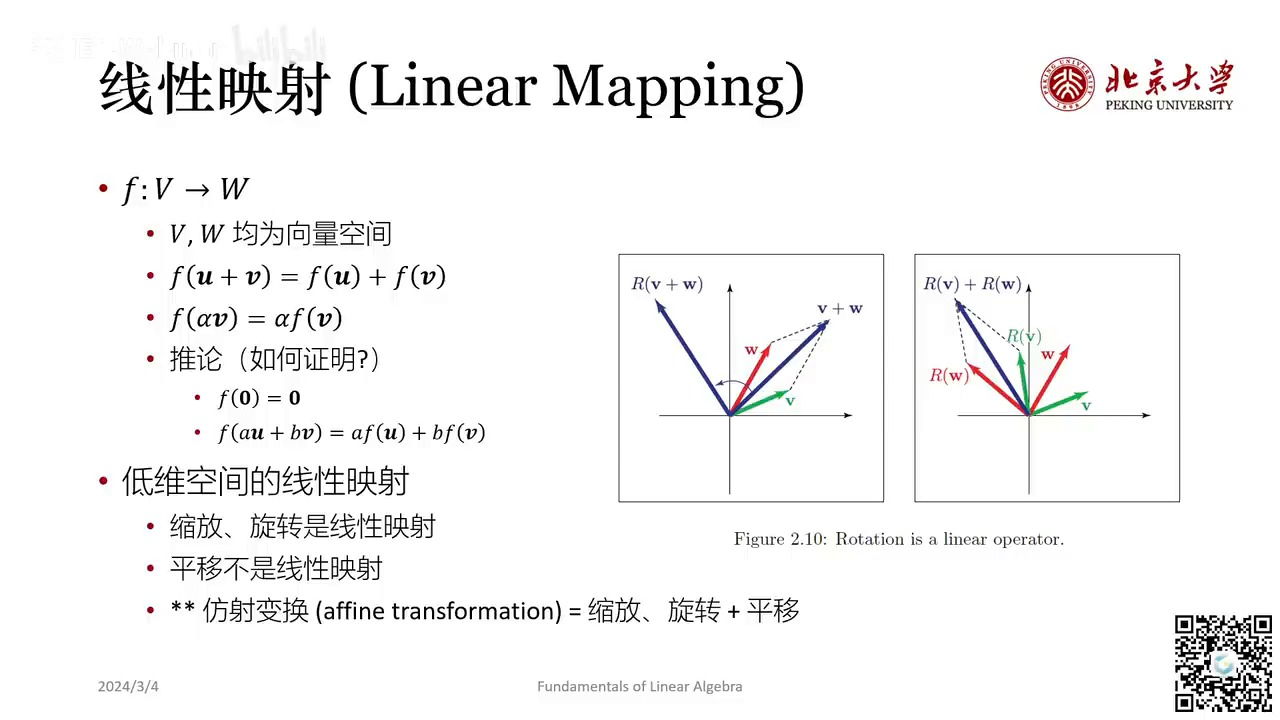
\includegraphics[width=0.92\textwidth]{figures/fig_24_linear_mapping.jpg}
\caption{线性映射的定义与“旋转是线性映射”的图示：先相加再旋转等于先旋转再相加\vtag}
\end{figure}
\srcnote{01:09:15--01:09:30}
\end{minipage}


然而图形学中平移与缩放、旋转同等重要，模型既要转也要移。因此需要引入仿射变换（affine transformation）：仿射变换等于缩放、旋转再加平移。后文的齐次坐标会把它重新纳入矩阵乘法的框架。

\begin{warningbox}{仿射变换不是线性变换}
仿射变换 $=$ 缩放、旋转 $+$ 平移，其中的平移部分不满足 $f(\boldsymbol 0)=\boldsymbol 0$。因此在普通坐标下，仿射变换无法写成单个矩阵乘向量的形式；它只有借助齐次坐标，才能在高一维的空间里表现为线性变换。
\end{warningbox}

\subsection{矩阵是线性映射的一种表示}

矩阵是什么？讲者在课件上打了两个标记：“二维数字阵列（2D array）”是错误的理解，“对线性映射的一种表示”才是正确的理解。他强烈推荐 3Blue1Brown 的线性代数系列视频，那里用动画直观地解释了矩阵的含义。

在这种理解下，矩阵运算的意义就清楚了：
\begin{itemize}
\item 矩阵与向量相乘，给出该向量在新的空间（经过矩阵对应的线性变换之后的空间）里的坐标；
\item 矩阵与矩阵相乘，表示对空间的多次相继变换的合成：先做一次线性映射再做另一次，等价于先把两次映射组合成一个，再作用于坐标；
\item $n\times n$ 的矩阵称为方阵，表示变换前后的空间具有相同的维度，其中的单位矩阵记作 $\boldsymbol E$。
\end{itemize}

\begin{importantbox}{本讲的核心视角}
矩阵不是一张数表，而是选定基之后线性映射的坐标表示。矩阵乘向量是“变换一个向量”，矩阵乘矩阵是“复合两个变换”。后面讨论转置、行列式、特征值时，都应先问它对应的线性变换有什么几何意义。
\end{importantbox}

\subsection{本章小结}

线性映射保持线性组合，因此可以由一张矩阵完整记录。旋转与缩放是线性的，平移不是，所以图形学需要仿射变换。下一章沿着“矩阵即变换”的视角，逐一解释矩阵的单目运算。

\section{矩阵的单目运算：每个运算的几何意义}

\noindent\begin{minipage}{\textwidth}
\begin{figure}[H]
\centering
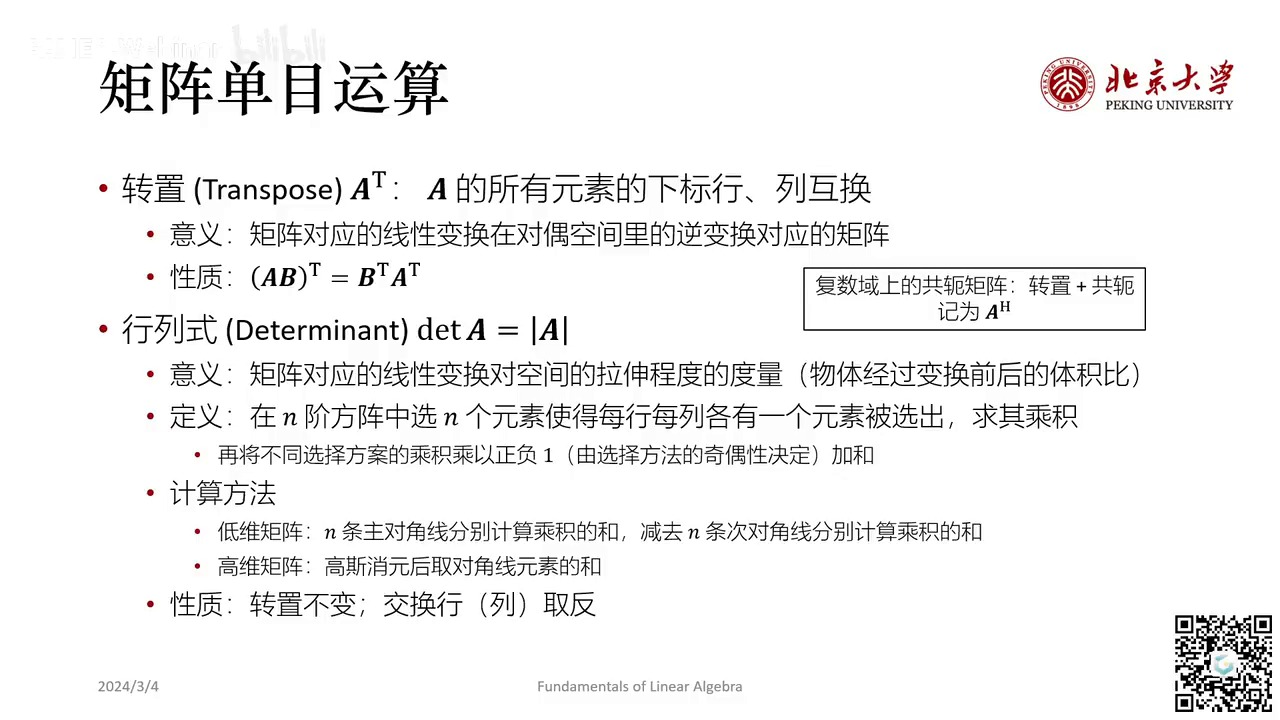
\includegraphics[width=0.92\textwidth]{figures/fig_25_matrix_unary.jpg}
\caption{矩阵单目运算：转置与行列式的意义、定义与性质\vtag}
\end{figure}
\srcnote{01:15:30--01:15:45}
\end{minipage}


\subsection{转置}

转置 $\boldsymbol A^{\mathsf T}$ 把 $\boldsymbol A$ 的所有元素的行下标与列下标互换，原来第一行第二列的元素变为第二行第一列。课件给出的意义是：矩阵对应的线性变换在对偶空间里的逆变换所对应的矩阵。讲者承认这一点涉及对偶空间，不太容易直观理解，感兴趣的读者可以课后了解。转置的性质为
\[
(\boldsymbol A\boldsymbol B)^{\mathsf T}=\boldsymbol B^{\mathsf T}\boldsymbol A^{\mathsf T}.
\]
\begin{itemize}
\item $\boldsymbol A,\boldsymbol B$：可相乘的矩阵；上标 $\mathsf T$：转置。
\end{itemize}
在复数域上，对应的概念是共轭转置：除了转置之外，还要把每个元素 $a+bi$ 改为 $a-bi$，记作 $\boldsymbol A^{\mathrm H}$。

\subsection{行列式：体积的伸缩比例}

既然旋转、缩放、拉伸都是线性变换，它们都在拉扯原来的图形，自然会改变图形的面积（二维）或体积（三维）。行列式 $\det\boldsymbol A=|\boldsymbol A|$ 的意义正是：矩阵对应的线性变换对空间的拉伸程度的度量，即物体经过变换前后的体积比。

定义上，在 $n$ 阶方阵中选 $n$ 个元素，使每行每列各有一个元素被选出，求其乘积；再将不同选择方案的乘积乘以正负 1 后加起来，正负号由选择方法的奇偶性决定。计算方法上，低维矩阵可以用“$n$ 条主对角线乘积之和减去 $n$ 条次对角线乘积之和”；高维矩阵则先用高斯消元消成三角形，再取对角线元素之积。讲者提醒，前一种算法仅适用于低维，并不像这里说的那么简单。性质包括：转置不改变行列式；交换两行（列）行列式取反。

\subsection{迹}

迹 $\operatorname{tr}\boldsymbol A$ 是矩阵对角线元素之和，其意义是矩阵的特征值之和。性质为
\[
\operatorname{tr}\boldsymbol A=\operatorname{tr}(\boldsymbol A^{\mathsf T}),\qquad
\operatorname{tr}(\boldsymbol A\boldsymbol B)=\operatorname{tr}(\boldsymbol B\boldsymbol A),\qquad
\operatorname{tr}(\boldsymbol A+\boldsymbol B)=\operatorname{tr}(\boldsymbol B+\boldsymbol A).
\]
\begin{itemize}
\item $\operatorname{tr}$：迹；$\boldsymbol A,\boldsymbol B$：方阵（第二式只要求 $\boldsymbol A\boldsymbol B$ 与 $\boldsymbol B\boldsymbol A$ 都有定义）。
\end{itemize}
第二条性质（乘积的迹可交换）在下一讲的矩阵求导中会反复出现。

\subsection{逆与伴随}

逆矩阵 $\boldsymbol A^{-1}$ 满足 $\boldsymbol A\boldsymbol A^{-1}=\boldsymbol E$。它的意义是矩阵对应的线性变换的逆变换的矩阵。求解方法有伴随矩阵法和高斯消元法：讲者描述了后者的操作，把单位矩阵接在待消元矩阵右边，当左边被消成单位矩阵时，右边恰好变成逆矩阵。性质为
\[
(\boldsymbol A\boldsymbol B)^{-1}=\boldsymbol B^{-1}\boldsymbol A^{-1},\qquad |\boldsymbol A|\,|\boldsymbol A^{-1}|=1 .
\]
\begin{itemize}
\item $\boldsymbol A,\boldsymbol B$：可逆方阵；$|\cdot|$：行列式。
\end{itemize}

伴随矩阵 $\boldsymbol A^{*}$ 由 $\boldsymbol A$ 的每个元素的代数余子式 $A_{ij}$ 构成：
\[
A_{ij}=(-1)^{i+j}M_{ij},\qquad \boldsymbol A\boldsymbol A^{*}=\boldsymbol A^{*}\boldsymbol A=|\boldsymbol A|\,\boldsymbol E ,
\]
\begin{itemize}
\item $M_{ij}$：余子式，即删去第 $i$ 行第 $j$ 列后的行列式的值；$A_{ij}$：代数余子式；$\boldsymbol E$：单位矩阵。
\end{itemize}
讲者指出，利用这条性质两边取行列式，就可以证明 $|\boldsymbol A|\,|\boldsymbol A^{-1}|=1$。

\noindent\begin{minipage}{\textwidth}
\begin{figure}[H]
\centering
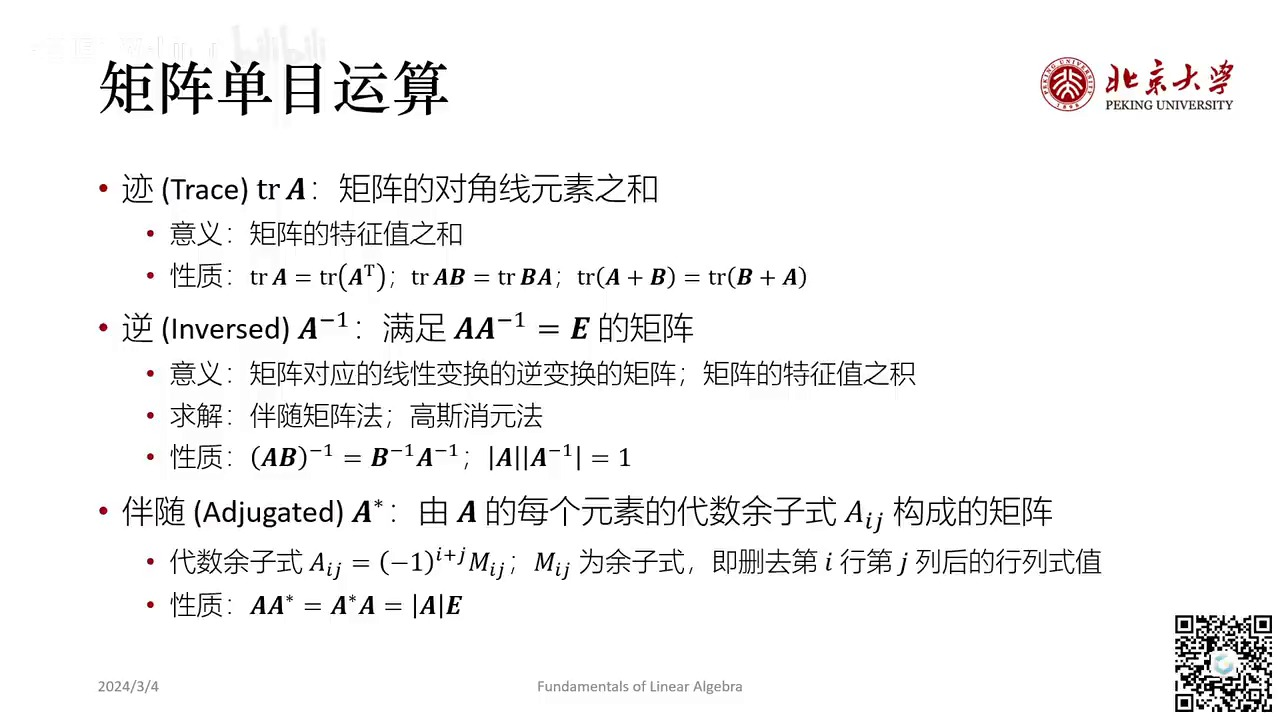
\includegraphics[width=0.92\textwidth]{figures/fig_26_trace_inverse_adjugate.jpg}
\caption{迹、逆与伴随矩阵的定义、意义与性质\vtag}
\end{figure}
\srcnote{01:18:15--01:18:30}
\end{minipage}


\subsection{本章小结}

转置、行列式、迹、逆、伴随都可以回到“矩阵即变换”来理解：行列式是体积比，逆是逆变换，迹是特征值之和。讲者坦言，这部分是对大一线性代数的快速回顾，目的是让读者知道后续会用到哪些知识。特征值本身则值得单独展开，因为它直接关系到数值算法是否收敛。

\section{特征值：变换在哪些方向上只是缩放}

\subsection{定义与求解}

对于某些向量 $\boldsymbol u$，若满足 $\lambda\boldsymbol u=\boldsymbol A\boldsymbol u$（$\boldsymbol A$ 为 $n$ 阶方阵），就称数 $\lambda$ 为特征值，这些向量称为特征向量。每个特征值对应的特征向量构成一个子空间：若 $\lambda\boldsymbol u=\boldsymbol A\boldsymbol u$，$\lambda\boldsymbol v=\boldsymbol A\boldsymbol v$，两式相加即得 $\lambda(\boldsymbol u+\boldsymbol v)=\boldsymbol A(\boldsymbol u+\boldsymbol v)$，满足向量空间的要求。

求解特征值需要
\[
(\lambda\boldsymbol E-\boldsymbol A)\boldsymbol u=\boldsymbol 0,\qquad |\lambda\boldsymbol E-\boldsymbol A|=0 ,
\]
\begin{itemize}
\item $\lambda$：待求的特征值；$\boldsymbol E$：$n$ 阶单位矩阵；$\boldsymbol u$：特征向量。
\end{itemize}
要使关于 $\boldsymbol u$ 的方程有非零解，系数矩阵的行列式必须为零，否则只有零解。这就是关于 $\lambda$ 的一元 $n$ 次方程。特征值的意义是：对于某些向量，特定线性变换的作用效果与数乘等价，即在这些方向上变换只是缩放。

\subsection{矩阵多项式}

把多项式 $f(x)$ 中的 $x$ 全部换成矩阵，就得到矩阵多项式：
\[
f(\boldsymbol A)=c_k\boldsymbol A^{k}+c_{k-1}\boldsymbol A^{k-1}+\cdots+c_1\boldsymbol A+c_0\boldsymbol E .
\]
\begin{itemize}
\item $c_0,\dots,c_k$：多项式系数；$\boldsymbol A^{k}$：$\boldsymbol A$ 的 $k$ 次幂；$\boldsymbol E$：单位矩阵，对应常数项。
\end{itemize}
它有两条好性质：若 $\lambda$ 是 $\boldsymbol A$ 的特征值，则 $f(\lambda)$ 必为 $f(\boldsymbol A)$ 的特征值；若 $\boldsymbol A$ 的特征值为 $\lambda_1,\dots,\lambda_n$，则 $f(\boldsymbol A)$ 的全部特征值由 $f(\lambda_1),\dots,f(\lambda_n)$ 给出。

\subsection{谱半径与条件数}

最大特征值（的绝对值）称为谱半径（spectral radius），最大与最小特征值之比称为条件数。讲者用矩阵多项式解释了谱半径为何是迭代算法的收敛判据：如果矩阵的最大特征值小于 1，随着幂次 $k$ 的升高，$\boldsymbol A^{k}$ 的最大特征值会一直下降。在迭代算法中，如果能证明谱半径一直在缩小，就说明算法收敛。条件数则衡量求解难度：条件数低的矩阵好解；最大特征值与最小特征值相差悬殊时，矩阵难解。

\noindent\begin{minipage}{\textwidth}
\begin{figure}[H]
\centering
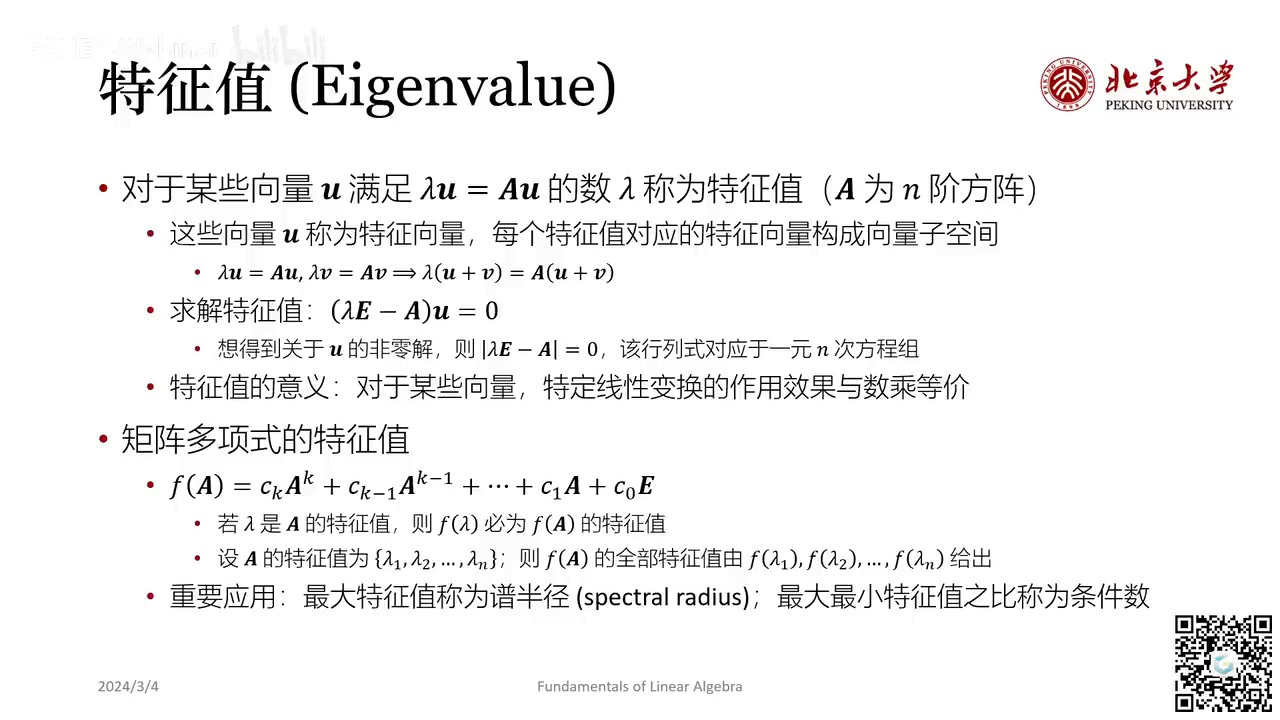
\includegraphics[width=0.92\textwidth]{figures/fig_27_eigenvalue.jpg}
\caption{特征值、矩阵多项式与谱半径、条件数\vtag}
\end{figure}
\srcnote{01:23:30--01:23:45}
\end{minipage}


\begin{knowledgebox}{特征值在后续讲次中的位置}
谱半径决定迭代法是否收敛，条件数决定线性系统是否好解。第十三讲“线性系统”会用到这两个量来分析迭代求解器；主成分分析与奇异值分解一讲也建立在特征值分解之上。
\end{knowledgebox}

\subsection{本章小结}

特征向量是变换只做缩放的方向，特征值是缩放的倍数。矩阵多项式把特征值的分析推广到 $\boldsymbol A^{k}$ 这类表达式上，进而得出谱半径与条件数两个数值判据。接下来，要讨论点乘、长度与角度这些几何量是如何引入的。

\section{度量、范数与内积：从距离到角度}

讲者在引入点乘之前，先为向量引入范数。范数（norm）可以理解为长度、大小或模长。为了说清楚范数，需要先说清楚“距离”。

\subsection{度量空间}

向量空间中的元素不能比大小。对集合 $V$，定义度量函数 $d:V\times V\to\mathbb R$，对任意 $x,y,z\in V$ 满足
\[
d(x,y)\ge 0,\quad d(x,y)=0\iff x=y,\quad d(x,y)=d(y,x),\quad d(x,z)\le d(x,y)+d(y,z).
\]
\begin{itemize}
\item $d$：度量函数，即“距离”；$x,y,z$：集合中的元素。
\end{itemize}
四条依次为非负性、不可区分者的同一性、对称性与三角不等式。讲者用地图上的两点作类比：距离不能小于零；距离为零时两点就是同一个点；从 $x$ 到 $z$ 不应比“先到中间点 $y$ 再到 $z$”更远。定义了度量函数的集合称为度量空间（metric space）。

\subsection{赋范向量空间}

赋范向量空间等于向量空间加上一个度量函数 $d(\boldsymbol u,\boldsymbol v)=\|\boldsymbol u-\boldsymbol v\|$。范数 $\|\cdot\|:V\to\mathbb R$ 需满足
\[
\|\boldsymbol u\|\ge 0,\ \ \|\boldsymbol u\|=0\iff\boldsymbol u=\boldsymbol 0,\qquad \|a\boldsymbol u\|=|a|\,\|\boldsymbol u\|,\qquad \|\boldsymbol u+\boldsymbol v\|\le\|\boldsymbol u\|+\|\boldsymbol v\| .
\]
\begin{itemize}
\item $\|\cdot\|$：范数；$a\in\mathbb R$：标量；$\boldsymbol u,\boldsymbol v\in V$。
\end{itemize}
三条分别称为正定性、正齐次性与次可加性（三角不等式）。其中正定性对应度量的“不可区分者的同一性”。

\noindent\begin{minipage}{\textwidth}
\begin{figure}[H]
\centering
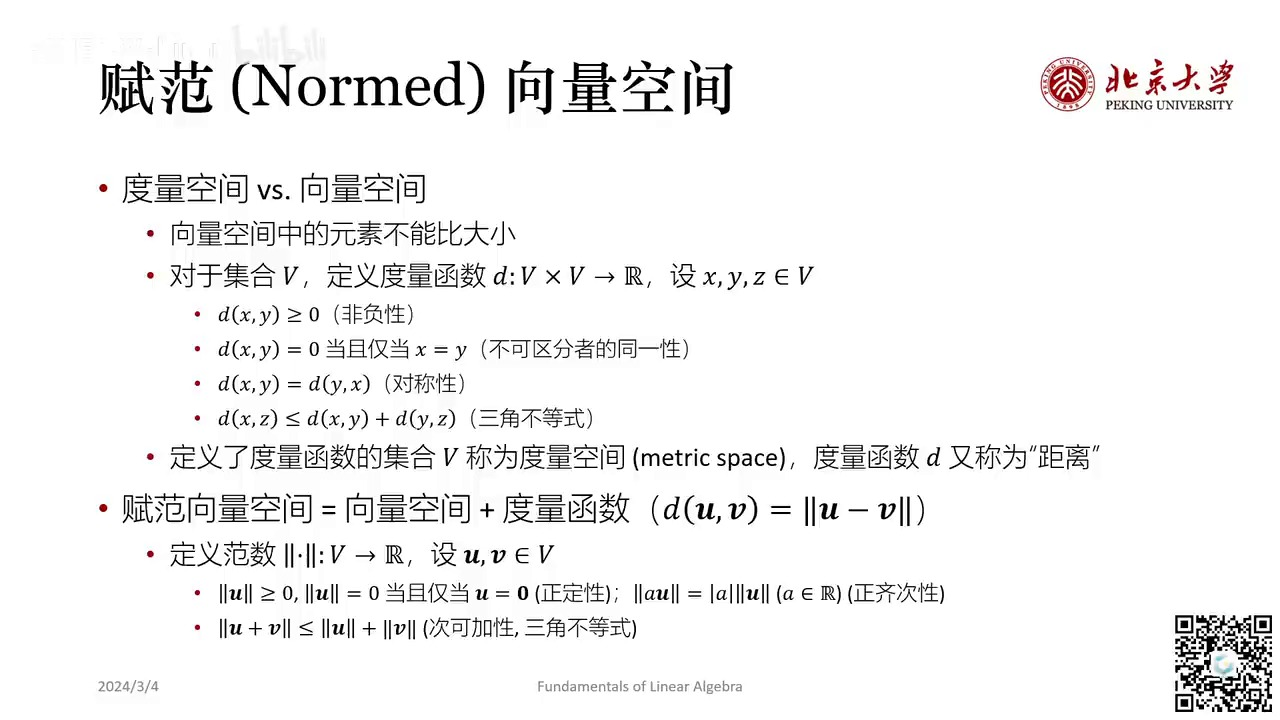
\includegraphics[width=0.92\textwidth]{figures/fig_28_normed_space.jpg}
\caption{赋范向量空间：度量空间的四条公理，以及范数的正定性、正齐次性与次可加性\vtag}
\end{figure}
\srcnote{01:27:45--01:28:00}
\end{minipage}


\subsection{内积空间}

内积是映射 $V\times V\to\mathbb R$，记作 $\langle\boldsymbol u,\boldsymbol v\rangle$，满足
\[
\langle\boldsymbol u,\boldsymbol v\rangle=\overline{\langle\boldsymbol v,\boldsymbol u\rangle},\quad
\langle\boldsymbol u,\boldsymbol v+\boldsymbol w\rangle=\langle\boldsymbol u,\boldsymbol v\rangle+\langle\boldsymbol u,\boldsymbol w\rangle,\quad
\langle\boldsymbol u,a\boldsymbol v\rangle=a\langle\boldsymbol u,\boldsymbol v\rangle,\quad
\langle\boldsymbol u,\boldsymbol u\rangle\ge 0 .
\]
\begin{itemize}
\item $\langle\cdot,\cdot\rangle$：内积；上划线：复共轭，在实数域上可以忽略；$a$：标量。
\end{itemize}
赋范线性空间与内积空间的关系是：内积可以诱导出度量 $d(\boldsymbol u,\boldsymbol u)=\langle\boldsymbol u,\boldsymbol u\rangle$（课件写法），范数只给出向量的长度，内积还给出向量的夹角。课件用一幅维恩图总结这些空间的包含关系：线性空间与度量空间是两个大集合，赋范向量空间位于二者交集中，内积空间又是赋范向量空间的一部分。

\noindent\begin{minipage}{\textwidth}
\begin{figure}[H]
\centering
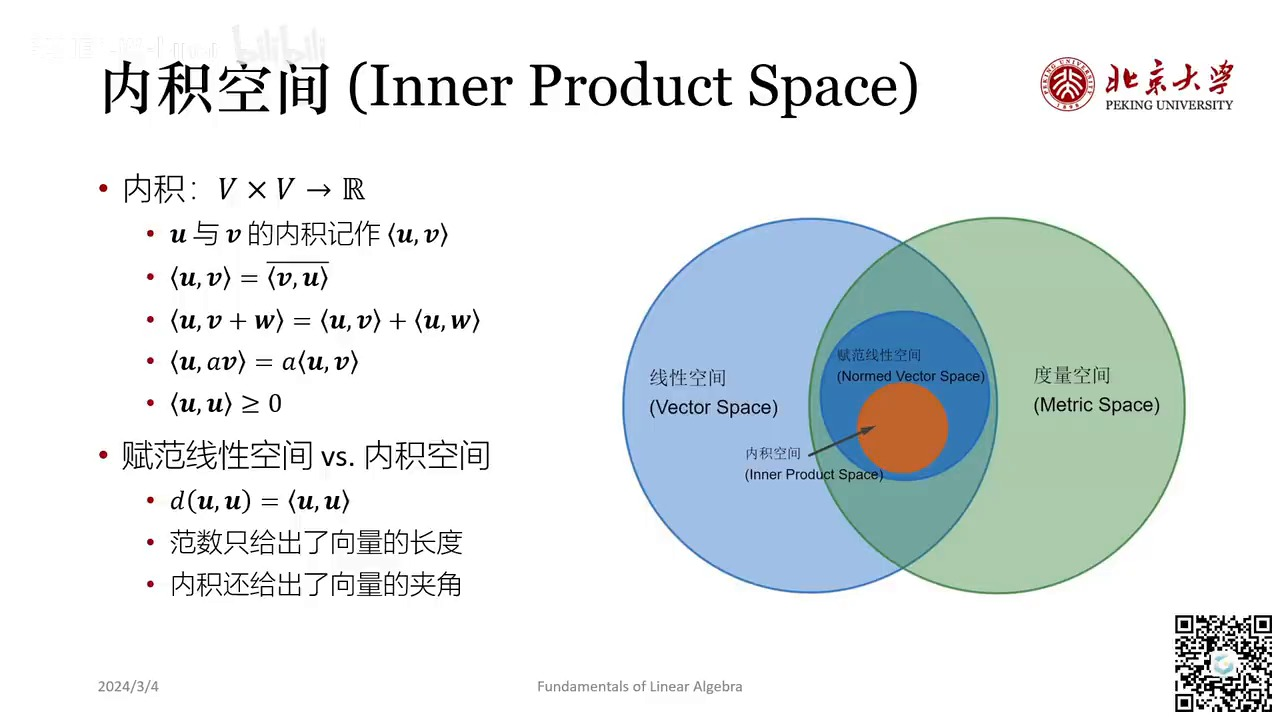
\includegraphics[width=0.92\textwidth]{figures/fig_29_spaces_venn.jpg}
\caption{线性空间、度量空间、赋范向量空间与内积空间的包含关系\vtag}
\end{figure}
\srcnote{01:30:00--01:30:15}
\end{minipage}


\subsection{夹角、正交与单位正交基}

内积如何给出夹角？定义两向量的夹角
\[
\theta_{\boldsymbol u\boldsymbol v}=\arccos\frac{\langle\boldsymbol u,\boldsymbol v\rangle}{\sqrt{\langle\boldsymbol u,\boldsymbol u\rangle\langle\boldsymbol v,\boldsymbol v\rangle}},
\]
\begin{itemize}
\item $\theta_{\boldsymbol u\boldsymbol v}$：夹角；分母是两向量长度之积，分子是内积。
\end{itemize}
当 $\cos\theta_{\boldsymbol u\boldsymbol v}=0$ 时称两向量正交。一组两两之间互相正交的基称为正交基底；模长均为 1 的基称为单位基底；两者合起来即单位正交基底。通过施密特（Schmidt）正交化与规范化，可以把任意一组基底变成单位正交基底。

单位正交基底让内积的计算变得简单。设 $\boldsymbol u=u_1\boldsymbol e_1+u_2\boldsymbol e_2+u_3\boldsymbol e_3$，$\boldsymbol v=v_1\boldsymbol e_1+v_2\boldsymbol e_2+v_3\boldsymbol e_3$，则
\[
\langle\boldsymbol u,\boldsymbol v\rangle=\langle u_1\boldsymbol e_1+u_2\boldsymbol e_2+u_3\boldsymbol e_3,\ v_1\boldsymbol e_1+v_2\boldsymbol e_2+v_3\boldsymbol e_3\rangle=u_1v_1+u_2v_2+u_3v_3 .
\]
\begin{itemize}
\item $\boldsymbol e_1,\boldsymbol e_2,\boldsymbol e_3$：单位正交基底；$u_i,v_i$：两向量在这组基下的坐标。
\end{itemize}
交叉项全部因正交而消失，平方项因单位长度而等于 1。

\subsection{单位正交变换与笛卡尔坐标系}

把一组单位正交基底变为另一组单位正交基底的线性变换，称为单位正交变换。它不改变任意两个向量的内积，因此保持长度与夹角。对应的单位正交矩阵 $\boldsymbol R$ 满足 $\boldsymbol R^{\mathsf T}=\boldsymbol R^{-1}$，对应于旋转以及镜像空间中的旋转，二者一起构成了全部单位正交矩阵。$\mathbb R^{n}$ 中的一组单位正交基底加上原点构成的坐标系称为笛卡尔坐标系（Cartesian coordinates），在其中内积就是坐标的点乘：$\langle\boldsymbol u,\boldsymbol v\rangle=\boldsymbol u^{\mathsf T}\boldsymbol v=\boldsymbol v^{\mathsf T}\boldsymbol u$。

\noindent\begin{minipage}{\textwidth}
\begin{figure}[H]
\centering
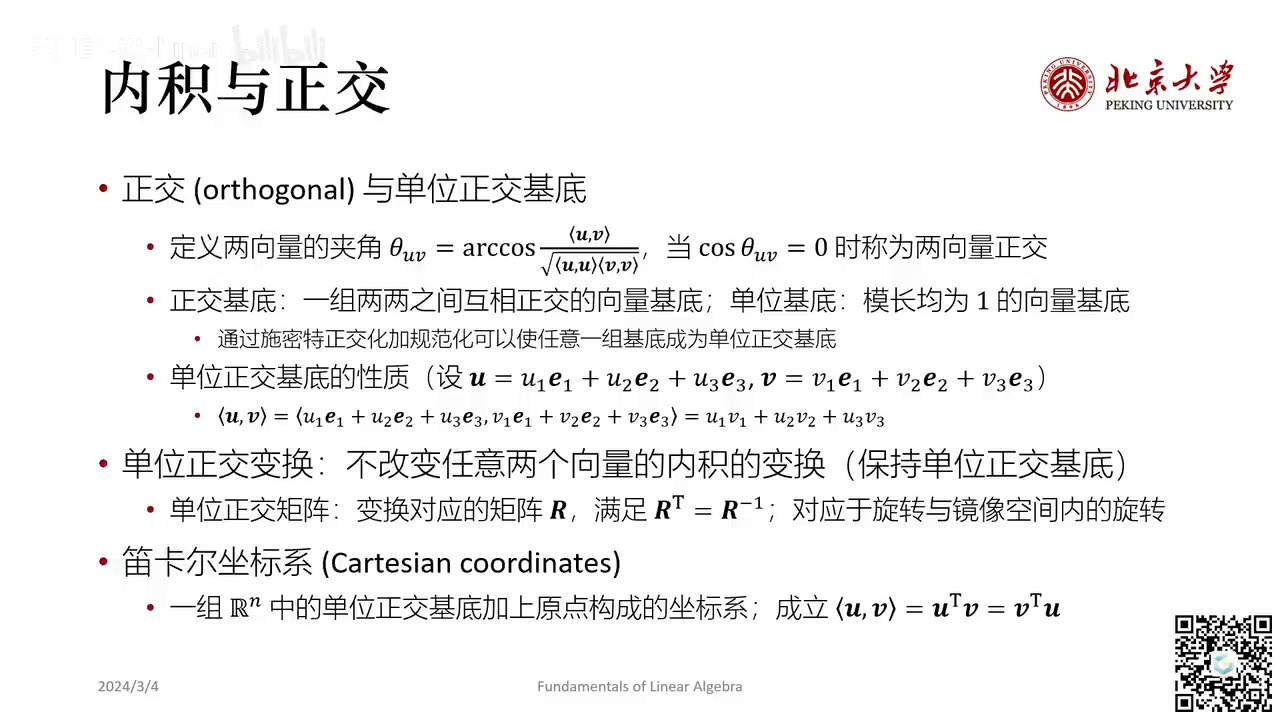
\includegraphics[width=0.92\textwidth]{figures/fig_30_orthogonality.jpg}
\caption{内积与正交：夹角定义、单位正交基底、单位正交变换与笛卡尔坐标系\vtag}
\end{figure}
\srcnote{01:33:30--01:33:45}
\end{minipage}


\subsection{幺正空间与函数空间}

幺正（unitary）空间在数学上又译为酉空间。讲者调侃“酉”这个字容易让人联想到地支，好像有十二种空间，其实它只是 unitary 的音译，他更喜欢物理学的译名“幺正”。

\begin{knowledgebox}{术语对照}
unitary 在数学文献中常译作“酉”，在物理文献中常译作“幺正”，二者指同一概念：酉空间即幺正空间，酉变换即幺正变换，酉矩阵即幺正矩阵。本讲义沿用讲者偏好的“幺正”。
\end{knowledgebox}
幺正空间是定义了内积的复数域 $\mathbb C$ 上的线性空间，内积通过埃尔米特（Hermite）函数给出；幺正变换把幺正空间中的单位正交基底（亦称规范正交基、标准正交基）变为单位正交基底，前面的单位正交变换是它在实数域 $\mathbb R$ 上的特例。

幺正空间最重要的用处在量子力学：波函数定义在复数域上，算子（operator）保持内积，这称为幺正性。讲者借此引出一个对图形学很重要的观点：函数空间是无限维的向量空间，线性算子是其上的线性变换，同样有特征值、内积等概念。今后如果遇到“函数的内积”乃至“函数的特征值”，不必恐慌，把函数理解为无穷维向量即可。他还补充：在图形学中，恰恰是把函数空间当作向量空间，才能把问题落到计算上。

\begin{importantbox}{函数即向量}
函数空间满足向量空间的公理，只是维度为无穷。函数的内积、函数空间上的线性算子及其特征值，都是有限维概念的直接推广。傅里叶变换与球谐函数一讲正是建立在这一视角上。
\end{importantbox}

\subsection{本章小结}

度量给出距离，范数给出长度，内积进一步给出角度。单位正交基让内积退化为坐标点乘，单位正交变换保持长度与角度，正是旋转与镜像。把这些概念推广到复数域和函数空间，就得到幺正变换与“函数即向量”的观点。下一章回到最具体的问题：在二维、三维中，缩放、剪切、旋转与平移的矩阵长什么样。

\section{低维变换矩阵与齐次坐标}

\subsection{二维线性变换}

二维线性变换把 $(x,y)$ 映射为
\[
\begin{pmatrix}a_{11}&a_{12}\\a_{21}&a_{22}\end{pmatrix}\begin{pmatrix}x\\y\end{pmatrix}=\begin{pmatrix}a_{11}x+a_{12}y\\a_{21}x+a_{22}y\end{pmatrix}.
\]
\begin{itemize}
\item $a_{ij}$：变换矩阵的元素；$(x,y)$：原坐标。
\end{itemize}
常见的三种二维变换为
\[
\begin{gathered}
\operatorname{scale}(s_x,s_y)=\begin{pmatrix}s_x&0\\0&s_y\end{pmatrix},\quad
\operatorname{shear}_x(s)=\begin{pmatrix}1&s\\0&1\end{pmatrix},\ \operatorname{shear}_y(s)=\begin{pmatrix}1&0\\s&1\end{pmatrix},\\
\operatorname{rotate}(\phi)=\begin{pmatrix}\cos\phi&-\sin\phi\\ \sin\phi&\cos\phi\end{pmatrix}.
\end{gathered}
\]
\begin{itemize}
\item $s_x,s_y$：$x$、$y$ 方向的缩放倍数；$s$：剪切系数；$\phi$：逆时针旋转角。
\end{itemize}
课件用一只钟表演示：缩放矩阵是对角矩阵，钟表在 $x$ 方向被压缩、在 $y$ 方向被拉长；剪切矩阵把钟表推成平行四边形，讲者在课上纠正了自己一处口误，沿 $x$ 方向的剪切对应的是第一行第二列放 $s$；旋转矩阵由三角函数给出，表示沿逆时针方向转过角度 $\phi$。

\noindent\begin{minipage}{\textwidth}
\begin{figure}[H]
\centering
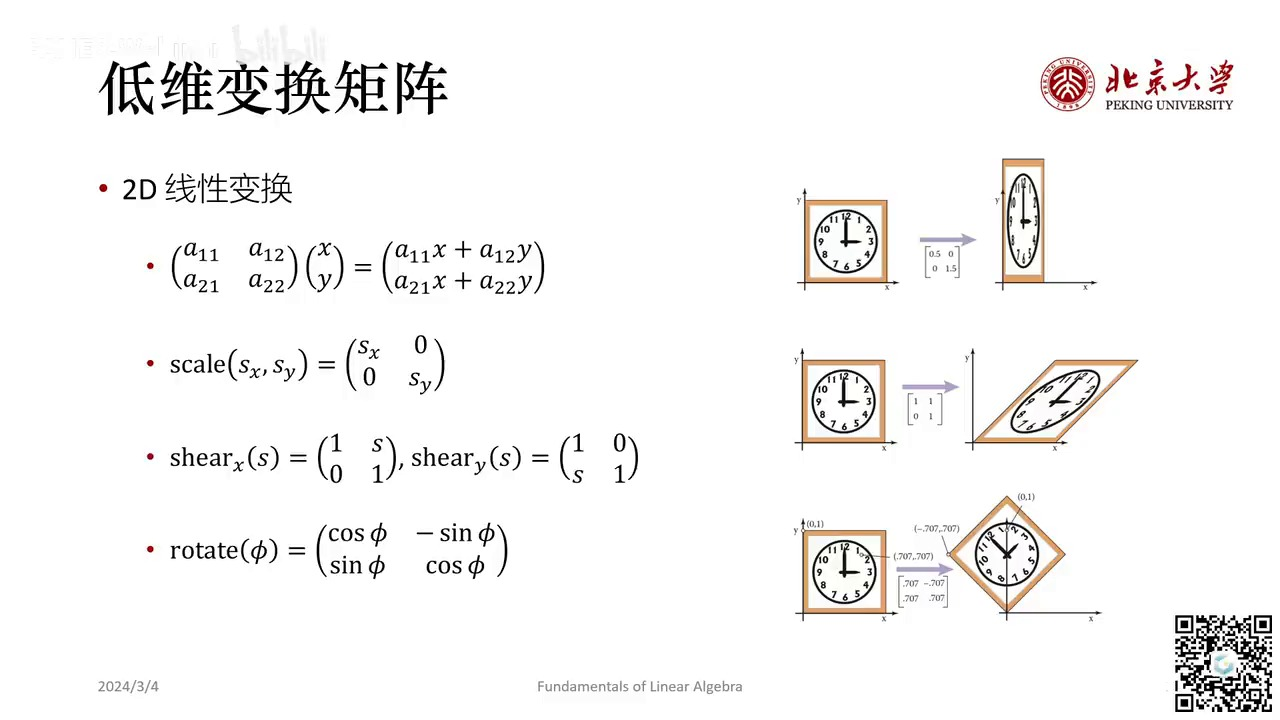
\includegraphics[width=0.92\textwidth]{figures/fig_31_2d_transforms.jpg}
\caption{二维缩放、剪切与旋转矩阵，以及它们作用在钟表上的效果\vtag}
\end{figure}
\srcnote{01:39:30--01:39:45}
\end{minipage}


\subsection{三维线性变换}

三维的缩放、剪切和绕 $z$ 轴的旋转为
\[
\begin{gathered}
\operatorname{scale}(s_x,s_y,s_z)=\begin{pmatrix}s_x&0&0\\0&s_y&0\\0&0&s_z\end{pmatrix},\quad
\operatorname{shear}_x(s_y,s_z)=\begin{pmatrix}1&s_y&s_z\\0&1&0\\0&0&1\end{pmatrix},\\
\operatorname{rotate}_z(\phi)=\begin{pmatrix}\cos\phi&-\sin\phi&0\\ \sin\phi&\cos\phi&0\\0&0&1\end{pmatrix}.
\end{gathered}
\]
\begin{itemize}
\item $s_x,s_y,s_z$：三个方向的缩放或剪切系数；$\phi$：绕 $z$ 轴的旋转角。
\end{itemize}
绕 $z$ 轴旋转与二维旋转完全相同，只是在第三行第三列多放了一个 1。但这并不完备：我们不能总是绕 $z$ 轴转，而希望绕任意轴旋转。课件给出的办法是先用一个旋转矩阵 $\boldsymbol R$ 把旋转轴转到 $z$ 轴，绕 $z$ 轴旋转后再转回去：
\[
\boldsymbol R^{\mathsf T}\begin{pmatrix}\cos\phi&-\sin\phi&0\\ \sin\phi&\cos\phi&0\\0&0&1\end{pmatrix}\boldsymbol R ,
\]
\begin{itemize}
\item $\boldsymbol R$：把旋转轴转到 $z$ 轴的变换矩阵；$\boldsymbol R^{\mathsf T}=\boldsymbol R^{-1}$：把 $z$ 轴转回原旋转轴。
\end{itemize}
讲者提到，旋转在第三讲会单独展开：四元数之所以在图形学中重要，是因为别的旋转表示方法都存在“锁”的问题（即万向节锁），会导致某些方向无法旋转。

\noindent\begin{minipage}{\textwidth}
\begin{figure}[H]
\centering
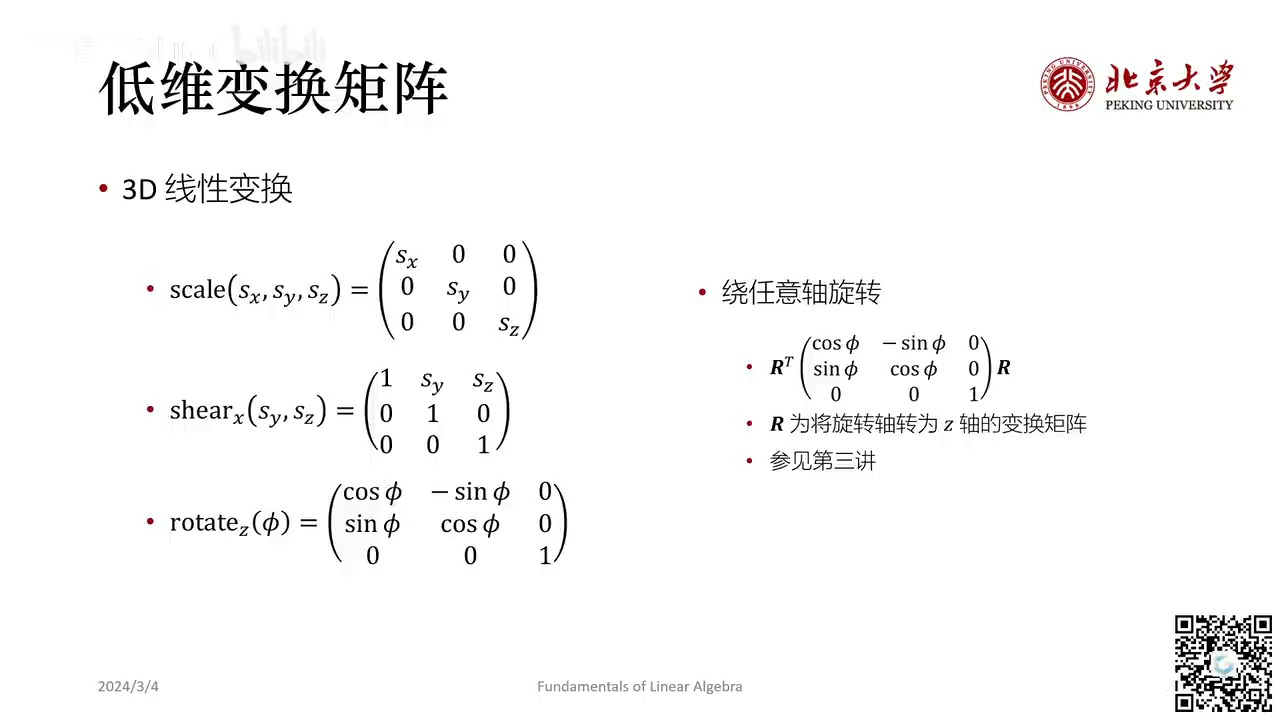
\includegraphics[width=0.92\textwidth]{figures/fig_32_3d_transforms.jpg}
\caption{三维缩放、剪切、绕 $z$ 轴旋转以及绕任意轴旋转的构造\vtag}
\end{figure}
\srcnote{01:40:45--01:41:00}
\end{minipage}


\subsection{齐次坐标：把平移纳入矩阵乘法}

前面一直没有解决平移问题。齐次（homogeneous）坐标的实质是用 $n+1$ 个数表示 $n$ 维坐标：
\[
(x,y,w)\to\left(\frac{x}{w},\frac{y}{w}\right),\qquad (x,y,z,w)\to\left(\frac{x}{w},\frac{y}{w},\frac{z}{w}\right).
\]
\begin{itemize}
\item $w$：齐次分量；箭头右侧为对应的普通 $n$ 维坐标。
\end{itemize}
齐次坐标等比例放缩不影响其表示的 $n$ 维坐标。讲者用课件的插图说明：二维笛卡尔坐标系中的点 $(1,2)$，在齐次坐标下可以写成 $(1,2,1)$、$(2,4,2)$ 或 $(3,6,3)$，它们在三维空间中位于同一条过原点的直线上，指向的是同一个点。

在齐次坐标下，二维仿射变换可以写成一次矩阵乘法：
\[
\begin{pmatrix}a_{11}&a_{12}&t_x\\a_{21}&a_{22}&t_y\\0&0&1\end{pmatrix}\begin{pmatrix}x\\y\\1\end{pmatrix}=\begin{pmatrix}a_{11}x+a_{12}y+t_x\\a_{21}x+a_{22}y+t_y\\1\end{pmatrix}.
\]
\begin{itemize}
\item 左上 $2\times2$ 块 $a_{ij}$：线性部分（缩放、剪切、旋转）；$t_x,t_y$：平移量；最后一行 $(0,0,1)$ 保持齐次分量为 1。
\end{itemize}
从乘法结果可以看出，平移是在线性变换完成之后进行的：先乘完线性部分，再加上 $t_x,t_y$。因此 Houdini、Blender 等商业图形软件的默认顺序是缩放 $\to$ 旋转 $\to$ 平移。

\noindent\begin{minipage}{\textwidth}
\begin{figure}[H]
\centering
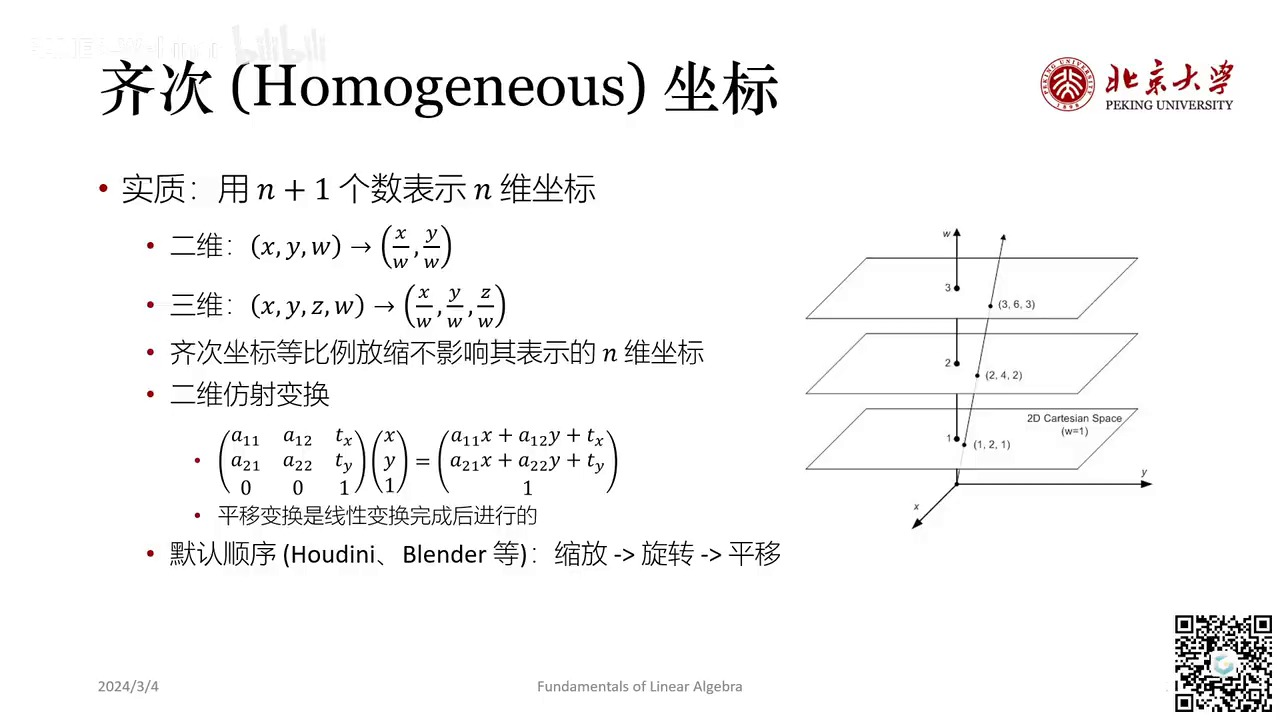
\includegraphics[width=0.92\textwidth]{figures/fig_33_homogeneous.jpg}
\caption{齐次坐标：用 $n+1$ 个数表示 $n$ 维坐标，等比例的齐次坐标指向同一点，仿射变换写成一次矩阵乘法\vtag}
\end{figure}
\srcnote{01:43:30--01:43:45}
\end{minipage}


\begin{warningbox}{变换顺序}
矩阵乘法一般不可交换，先旋转再平移与先平移再旋转得到不同结果。齐次坐标下仿射矩阵的结构决定了“先线性变换、后平移”；在软件之间迁移模型变换时，需要确认各自的默认顺序。
\end{warningbox}

\subsection{本章小结}

二维、三维的缩放、剪切、旋转都是小方阵；绕任意轴旋转可以通过“转到 $z$ 轴—旋转—转回”构造；齐次坐标多用一个分量，把平移也变成矩阵乘法，于是整条仿射变换链都能用矩阵连乘表示。至此讨论的都是“矩阵作用于向量”，下一章讨论“矩阵本身被变换”。

\section{矩阵的变换、二次型与正定矩阵}

\subsection{矩阵的变换不是线性变换}

讲者首先区分两个概念：矩阵是线性变换的表示，所以“矩阵的变换”其实是线性变换的“变换”，两者不是一回事。最重要的两种矩阵变换是相似变换与合同变换。

\paragraph{相似变换。}若存在可逆矩阵 $\boldsymbol P$ 使
\[
\boldsymbol P^{-1}\boldsymbol A\boldsymbol P=\boldsymbol B ,
\]
\begin{itemize}
\item $\boldsymbol P$：可逆矩阵，可理解为基变换；$\boldsymbol A,\boldsymbol B$：同一线性变换在两组基下的矩阵，
\end{itemize}
就称矩阵 $\boldsymbol A,\boldsymbol B$ 相似，记作 $\boldsymbol A\sim\boldsymbol B$。意义是：$\boldsymbol A$ 与 $\boldsymbol B$ 可以看作同一个线性变换在不同基底下的表象。相似对角化：当存在 $n$ 个线性无关的特征向量时，可以把矩阵相似为一个对角矩阵，意思是在某个特殊的基底下，矩阵对应的线性变换等价于纯缩放变换。

\paragraph{合同变换。}若存在可逆矩阵 $\boldsymbol C$ 使
\[
\boldsymbol C^{\mathsf T}\boldsymbol A\boldsymbol C=\boldsymbol B ,
\]
\begin{itemize}
\item $\boldsymbol C$：可逆矩阵；$\boldsymbol C^{\mathsf T}$：其转置（相似变换中的 $\boldsymbol P^{-1}$ 在这里换成了转置），
\end{itemize}
就称矩阵 $\boldsymbol A,\boldsymbol B$ 合同，记作 $\boldsymbol A\approx\boldsymbol B$。意义是：$\boldsymbol A$ 与 $\boldsymbol B$ 可以看作同一个二次型在不同基底下的表象。

\noindent\begin{minipage}{\textwidth}
\begin{figure}[H]
\centering
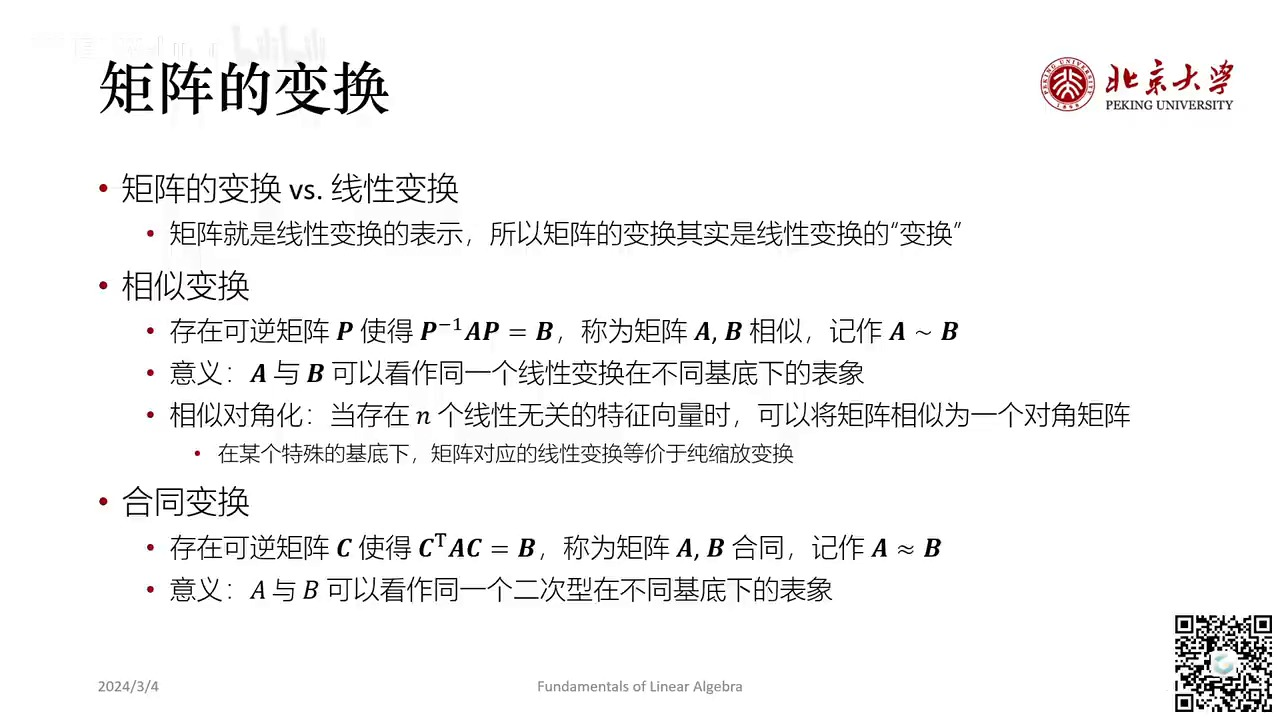
\includegraphics[width=0.92\textwidth]{figures/fig_34_similarity_congruence.jpg}
\caption{矩阵的变换：相似变换对应同一线性变换的不同表象，合同变换对应同一二次型的不同表象\vtag}
\end{figure}
\srcnote{01:46:15--01:46:30}
\end{minipage}


\subsection{二次型}

二次型（quadratic form）是 $n$ 个变量的二次齐次多项式。课件以圆锥曲线为例：
\[
Ax^2+2Bxy+Cy^2+2Dx+2Ey+F=0
\iff
\begin{pmatrix}x&y&1\end{pmatrix}\begin{pmatrix}A&B&D\\B&C&E\\D&E&F\end{pmatrix}\begin{pmatrix}x\\y\\1\end{pmatrix}=0 .
\]
\begin{itemize}
\item $A,\dots,F$：圆锥曲线的系数；$(x,y,1)$：点的齐次坐标；中间的对称矩阵即二次型矩阵。
\end{itemize}
一般形式写作 $\boldsymbol x^{\mathsf T}\boldsymbol A\boldsymbol x=0$，其中 $\boldsymbol x$ 是坐标，$\boldsymbol A$ 是二次型矩阵。

合同变换对二次型做了什么？做坐标变换 $\boldsymbol x=\boldsymbol C\boldsymbol x'$ 之后：
\[
\boldsymbol x^{\mathsf T}(\boldsymbol C^{\mathsf T}\boldsymbol A\boldsymbol C)\boldsymbol x=0\Rightarrow
\boldsymbol x^{\mathsf T}\boldsymbol C^{\mathsf T}\boldsymbol A\boldsymbol C\boldsymbol x=0\Rightarrow
(\boldsymbol C\boldsymbol x)^{\mathsf T}\boldsymbol A(\boldsymbol C\boldsymbol x)=0 .
\]
\begin{itemize}
\item $\boldsymbol C$：基变换矩阵；$\boldsymbol C\boldsymbol x$：变换后的坐标。
\end{itemize}
意义是：基底改变以后，为保持二次型（即曲线本身）不变，中间的矩阵也要相应地变成 $\boldsymbol C^{\mathsf T}\boldsymbol A\boldsymbol C$，这就是合同变换后的二次型系数。

最基础的应用是把任意朝向的椭圆方程化为标准形式。原方程有 $2Bxy$、$2Dx$、$2Ey$ 等交叉项；经过合同变换，可以化为
\[
\frac{x^2}{a^2}+\frac{y^2}{b^2}=1\iff
\begin{pmatrix}x&y&1\end{pmatrix}\begin{pmatrix}1/a^2&0&0\\0&1/b^2&0\\0&0&-1\end{pmatrix}\begin{pmatrix}x\\y\\1\end{pmatrix}=0 ,
\]
\begin{itemize}
\item $a,b$：椭圆的两个半轴长；中间矩阵只剩对角元。
\end{itemize}

\noindent\begin{minipage}{\textwidth}
\begin{figure}[H]
\centering
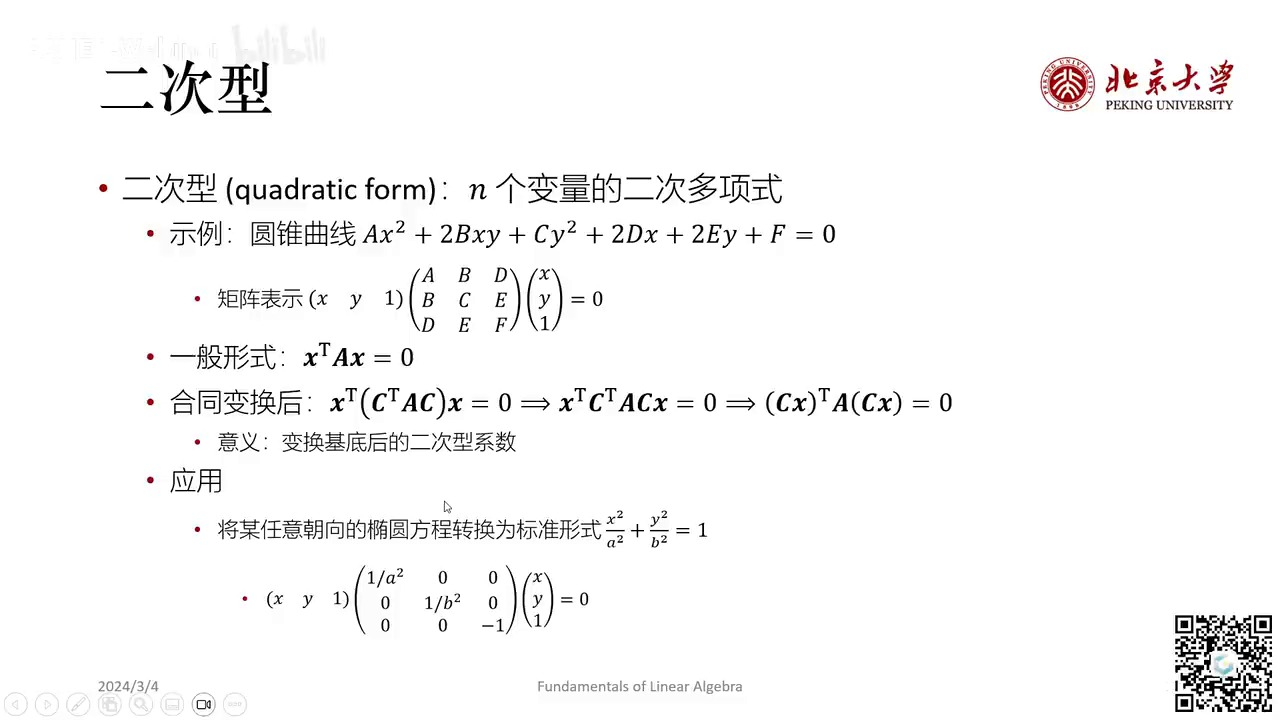
\includegraphics[width=0.92\textwidth]{figures/fig_35_quadratic_form.jpg}
\caption{二次型：圆锥曲线的矩阵表示、合同变换的意义，以及把任意朝向的椭圆化为标准形\vtag}
\end{figure}
\srcnote{01:49:00--01:49:15}
\end{minipage}


\subsection{正定矩阵与 Hessian}

满足 $\boldsymbol x^{\mathsf T}\boldsymbol A\boldsymbol x>0\ (\boldsymbol x\neq\boldsymbol 0)$ 的矩阵称为正定（positive definite）矩阵，其意义是可以构建恒取正值的二次型。二次型与分析相结合：二元可微函数 $f(x,y)$ 的二阶微分为
\[
\begin{pmatrix}\mathrm dx&\mathrm dy\end{pmatrix}
\begin{pmatrix}\dfrac{\partial^2 f}{\partial x^2}&\dfrac{\partial^2 f}{\partial x\partial y}\\[2mm]\dfrac{\partial^2 f}{\partial x\partial y}&\dfrac{\partial^2 f}{\partial y^2}\end{pmatrix}
\begin{pmatrix}\mathrm dx\\ \mathrm dy\end{pmatrix},
\]
\begin{itemize}
\item $\mathrm dx,\mathrm dy$：自变量的微小变化，决定了方向；中间矩阵：二阶偏导组成的 Hessian 矩阵，对角元为 $\partial^2 f/\partial x^2$、$\partial^2 f/\partial y^2$，非对角元为 $\partial^2 f/\partial x\partial y$。
\end{itemize}
它给出了沿任意方向的二阶导数。如果这个二次型恒正，说明沿任何方向的二阶导数都是正的；反之，若存在某个方向二阶导数不恒大于零，那个点就不可能是极小值点。讲者指出，这正是我们在做优化或解方程时要求正定性的原因。

正定矩阵的特征值全为正数，但逆命题不成立。满足 $\boldsymbol x^{\mathsf T}\boldsymbol A\boldsymbol x\ge 0\ (\boldsymbol x\neq\boldsymbol 0)$ 的矩阵称为半正定矩阵。

\subsection{实对称矩阵}

刚才 Hessian 矩阵不仅是正定的，还是对称的：其转置与自身相同。实数域上满足 $\boldsymbol A^{\mathsf T}=\boldsymbol A$ 的矩阵称为实对称矩阵，其性质是可以被正交矩阵对角化。对实对称矩阵而言，前面不成立的逆命题成立了：只要特征值全为正数，它就是正定的。这是判断实对称矩阵是否正定的常用办法。复数域上对应的是埃尔米特（Hermitian）矩阵，满足 $\boldsymbol A^{\mathrm H}=\boldsymbol A$。

\noindent\begin{minipage}{\textwidth}
\begin{figure}[H]
\centering
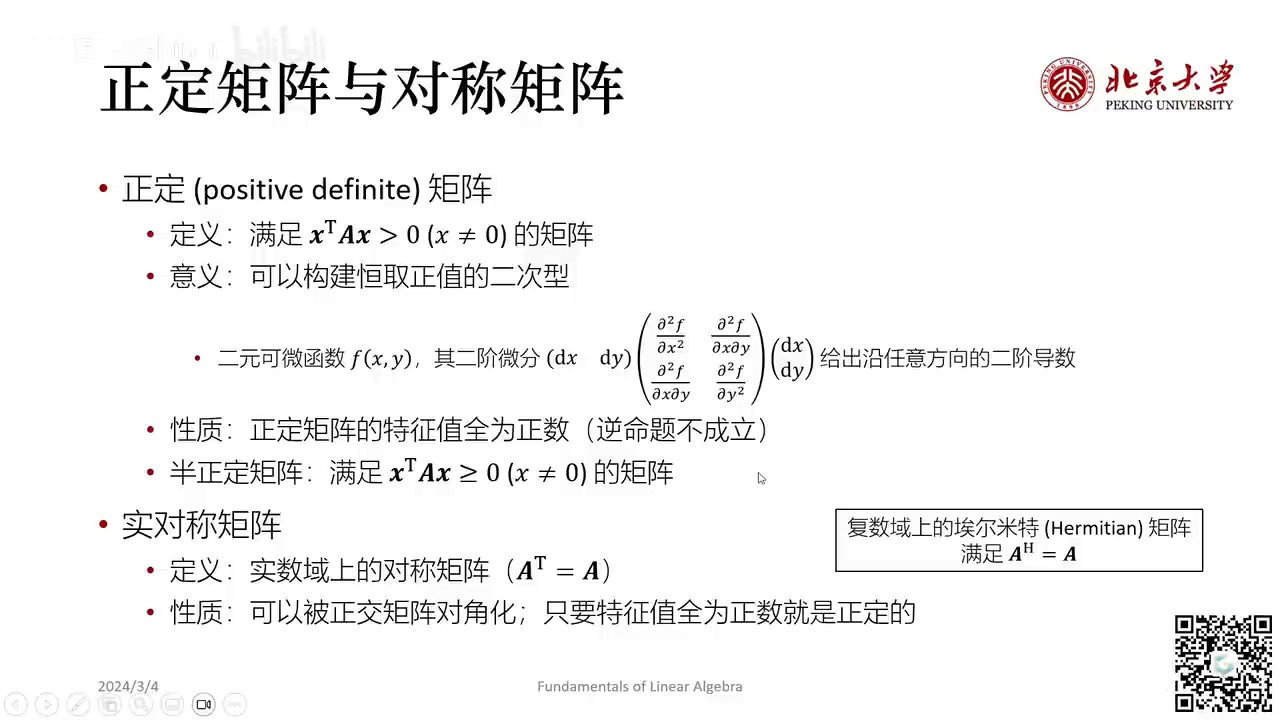
\includegraphics[width=0.92\textwidth]{figures/fig_36_positive_definite.jpg}
\caption{正定矩阵、二元函数二阶微分的二次型表示，以及实对称矩阵的性质\vtag}
\end{figure}
\srcnote{01:53:30--01:53:45}
\end{minipage}


\begin{importantbox}{正定性与极小值}
函数在某点的 Hessian 正定，意味着沿任意方向的二阶导数为正，该点才可能是极小值点。对实对称矩阵，“正定”等价于“特征值全为正”。这条判据会在优化基础、线性系统（如共轭梯度法要求系数矩阵对称正定）等讲次中反复出现。
\end{importantbox}

\begin{warningbox}{一个常见的混淆}
“正定矩阵的特征值全为正”对一般矩阵只是必要条件，逆命题不成立；只有限定为实对称（或埃尔米特）矩阵时，“特征值全为正”才足以判定正定。
\end{warningbox}

\subsection{本章小结}

相似变换和合同变换都在“换基”，前者保持线性变换，后者保持二次型。二次型把圆锥曲线、二阶导数统一为 $\boldsymbol x^{\mathsf T}\boldsymbol A\boldsymbol x$ 的形式，正定性则刻画了“沿任何方向都向上弯”，这正是极小值与可解性的前提。矩阵分解、范数、矩阵求导与张量这几部分留给下一讲。

\section{总结与延伸}

\subsection{讲者的收尾}

倪星宇在结尾说明，本讲内容基本是对线性代数的快速回顾，目的不是从头教学，而是让读者知道图形学到底要用到哪些线性代数知识；下一讲的矩阵求导、范数与张量部分，可能是许多读者在大一课程中没有系统接触过的。他再次强调了函数空间的观点：函数求特征值的结论很容易记，也比较“想当然”；在图形学中，反而要把函数空间看成向量空间才能计算。掌握这些数学证明，会让后续的学习研究更加轻车熟路；即使暂时不掌握，知道结论也能使用。由于本讲没有讲完，作业将在下一讲布置。

\subsection{本讲的知识主线}

\begin{center}
\begin{tabular}{p{0.22\textwidth}p{0.34\textwidth}p{0.34\textwidth}}
\toprule
概念 & 定义的核心 & 在图形学中的作用 \\
\midrule
向量空间 & 满足八条公理的集合 & 位置、法向、颜色、网格状态、函数 \\
基与维度 & 线性无关向量的最大个数 & 从三维坐标到 $10^6$--$10^7$ 维模拟状态 \\
线性映射/矩阵 & 保持线性组合的映射及其坐标表示 & 缩放、剪切、旋转与变换复合 \\
行列式/迹/逆 & 体积比、特征值之和、逆变换 & 判断可逆性、矩阵求导中的迹技巧 \\
特征值 & $\lambda\boldsymbol u=\boldsymbol A\boldsymbol u$ & 谱半径判断收敛、条件数衡量难度 \\
内积与正交 & 给出长度与夹角 & 单位正交基、旋转矩阵 $\boldsymbol R^{\mathsf T}=\boldsymbol R^{-1}$ \\
齐次坐标 & 用 $n+1$ 个数表示 $n$ 维点 & 平移纳入矩阵乘法，默认缩放—旋转—平移 \\
二次型与正定 & $\boldsymbol x^{\mathsf T}\boldsymbol A\boldsymbol x$ 恒正 & 圆锥曲线标准化、极小值判据 \\
\bottomrule
\end{tabular}
\end{center}

\subsection{讲义作者的归纳}

以下是本讲义的整理，而非讲者原话。本讲的线性代数可以压缩成三层：第一层是“对象”，向量空间与基告诉我们图形学的数据可以统一看作向量，而维度从 3 跨到上千万；第二层是“作用”，矩阵是线性映射的表示，行列式、迹、特征值都是变换的几何属性，齐次坐标把仿射变换也纳入矩阵；第三层是“几何结构”，内积引入长度与角度，二次型与正定性刻画曲面的弯曲方向。陈宝权老师开场提出的世界模拟器，从几何重建到物理仿真，其底层计算都要落到这三层上。

\subsection{留给读者的问题}

\begin{itemize}
\item 为颜色空间定义合适的加法与数乘，检验它是否满足向量空间的八条公理。
\item 由线性映射的定义证明 $f(\boldsymbol 0)=\boldsymbol 0$ 与 $f(a\boldsymbol u+b\boldsymbol v)=af(\boldsymbol u)+bf(\boldsymbol v)$。
\item 为什么实对称矩阵“特征值全为正”就足以说明它正定，而一般矩阵不行？
\item 函数空间是无穷维向量空间。函数的内积应如何定义，才能满足内积的四条性质？
\end{itemize}

\end{document}
